\documentclass[eng,printmode,oneside]{mgr}
%opcje klasy dokumentu mgr.cls zostaly opisane w dolaczonej instrukcji

%ponizej deklaracje uzycia pakietow, usunac to co jest niepotrzebne
\usepackage{polski} %przydatne podczas skladania dokumentow w j. polskim
%\usepackage[polish]{babel}%alternatywnie do pakietu polski, wybrac jeden z nich
\usepackage[utf8]{inputenc} %kodowanie znakow, zalezne od systemu
\usepackage[T1]{fontenc} %poprawne skladanie polskich czcionek


%listingi
\usepackage{listings}
\usepackage{color}
\usepackage[usenames,dvipsnames]{xcolor}
%\usepackage{mathdots}

\definecolor{zielony}{rgb}{0,0.6,0}
\definecolor{innyZielony}{rgb}{0.5,0.7,0}

\definecolor{mygreen}{rgb}{0,0.6,0}
\definecolor{mygray}{rgb}{0.5,0.5,0.5}
\definecolor{mymauve}{rgb}{0.58,0,0.82}
\definecolor{xmlString}{RGB}{200,16,0}
\definecolor{violet}{RGB}{80,33,97}
\definecolor{darkblue}{RGB}{15,1,255}
\definecolor{darkred}{RGB}{161,0,0}
\definecolor{greenJSP}{RGB}{25,154,12}
\definecolor{violetJSP}{RGB}{109,18,56}

\lstset{ %
  language=Java,
  backgroundcolor=\color{white},   % choose the background color; you must add \usepackage{color} or \usepackage{xcolor}
  basicstyle=\footnotesize,        % the size of the fonts that are used for the code
  breakatwhitespace=false,         % sets if automatic breaks should only happen at whitespace
  breaklines=true,                 % sets automatic line breaking
  captionpos=b,                    % sets the caption-position to bottom
  commentstyle=\color{mygray},    % comment style
  deletekeywords={...},            % if you want to delete keywords from the given language
  extendedchars=true,              % lets you use non-ASCII characters; for 8-bits encodings only, does not work with UTF-8
  frame=single,                    % adds a frame around the code
  keepspaces=true,                 % keeps spaces in text, useful for keeping indentation of code (possibly needs columns=flexible)
  keywordstyle=\color{darkred}\textbf,       % keyword style
  morekeywords={},            % if you want to add more keywords to the set
  numbers=left,                    % where to put the line-numbers; possible values are (none, left, right)
  numbersep=5pt,                   % how far the line-numbers are from the code
  numberstyle=\tiny\color{mygray}, % the style that is used for the line-numbers
  rulecolor=\color{black},         % if not set, the frame-color may be changed on line-breaks within not-black text (e.g. comments (green here))
  showspaces=false,                % show spaces everywhere adding particular underscores; it overrides 'showstringspaces'
  showstringspaces=false,          % underline spaces within strings only
  showtabs=false,                  % show tabs within strings adding particular underscores
  stepnumber=1,                    % the step between two line-numbers. If it's
  % 1, each line will be numbered
  stringstyle=\color{blue},     % string literal style
  tabsize=2,                       % sets default tabsize to 2 spaces
  %identifierstyle=\color{blue},
  %title=\lstname,                   % show the filename of files included with
  % \lstinputlisting; also try caption instead of title
  keywordstyle=[3]{\color{darkblue!50!black}},
  keywordstyle=[4]{\color{greenJSP!50!black}\textbf},
  keywordstyle=[5]{\color{violetJSP!50!black}\textbf},
  escapeinside={(*@}{@*)}
}
\newcommand{\CodeSymbol}[1]{\textcolor{greenJSP}{#1}\textbf}

\usepackage{url}

%kolor do komentarzy, uwag, przypomnienie
\definecolor{komentarz}{rgb}{1,0,0}
 
%pakiety do grafiki
\usepackage{graphicx}
\usepackage{subfigure}
\usepackage{psfrag}
\usepackage[justification=centering]{caption}
\usepackage{wrapfig}
\usepackage{lipsum}

%pakiety dodajace duzo dodatkowych polecen matematycznych
\usepackage{amsmath} 
\usepackage{amsfonts}

%pakiety wspomagajace i poprawiajace skladanie tabel
\usepackage{supertabular}
\usepackage{array}
\usepackage{tabularx}
\usepackage{hhline}

%pakiet wypisujacy na marginesie etykiety rownan i rysunkow zdefiniowanych przez \label{}, chcac wygenerowac finalna wersje dokumentu wystarczy usunac 
%ponizsza linie
%\usepackage{showlabels}
\sloppy

%definicje wlasnych polecen
\newcommand{\R}{I\!\!R} %symbol liczb rzeczywistych, dziala tylko w trybie matematycznym
\newtheorem{theorem}{Twierdzenie}[section] %nowe otoczenie do skladania twierdzen

%dane do zlozenia strony tytulowej
\title{System monitoringu lokalizacji przesyłek kurierskich}
\engtitle{English title ŁŁĄŚŹĆŻÓ łąśćźżóę Ę}
\author{Monika Strachowska}
\supervisor{dr hab. inz. Imie Nazwisko Prof. PWr, I-6}
%\guardian{dr hab. inz. Imie Nazwisko Prof. PWr, I-6} %nie uzywac jesli opiekun jest ta sama osoba co prowadzacy prace

%\date{2008} %standardowo u dolu strony tytulowej umieszczany jest biezacy rok, to polecenie pozwala wstawic dowolny rok

%ponizej jest lista kierunkow i specjalnosci na wydziale elektroniki, nalezy wybrac wlasciwe lub dopisac jesli nie ma odpowiednich
\field{Automatyka i Robotyka (AIR)}
\specialisation{Systemy informatyczne w automatyce (ASI)}

%tutaj zaczyna sie wlasciwa tresc dokumentu
\begin{document}

\bibliographystyle{plabbrv} %tylko gdy uzywamy BibTeXa, ustawia polski styl bibliografii

\maketitle %polecenie generujace strone tytulowa


\tableofcontents %spis tresci

%ponizej znajduje sie przykladowa tresc dalszej czesci dokumentu, zainteresowanych zachecam do rozszyfrowania frazy "Lorem ipsum" :)
\chapter{Wstęp i cel pracy}

Współcześnie coraz więcej osób korzysta z możliwości zakupów przez internet,
niesie to za sobą wiele korzyści. Często zakupiony towar jest tańszy, unikalny,
bądź niedostępny w stacjonarnym sklepie czy po prostu jest to wygodniejsza forma
zakupów. Oprócz wyżej wymienionych zakupów istotnym towarem przewożonym
są dokumenty, często szybko potrzebne. Z tych powodów ludzie zamawiający usługi 
kurierskie chcieliby dostać jak najwyższą jakość. Zwiększenie jakości tej
usługi może nastąpić poprzez skrócenie czasu dostarczenia przesyłki(co
fizycznie już jest nie osiągalne), tańszy jej koszt, czy na przykład możliwość
sprawdzenia, w jakim dokładnie miejscu ona się znajduje. Dokładna lokalizacja
przesyłki - taka funkcjonalność usługi kurierskiej nie należy do jakości
wymaganej i koniecznej, ale znacznie podniesie prestiż firmy
kurierskiej, która zdecyduje się na taką dodatkową funkcjonalność. Z punktu
widzenia klienta odczuwany jest komfort informacji, gdzie jest przesyłka, dzięki
temu klient może zaplanować sobie dzień, w którym nastąpi dostarczenie. 

Przedstawiany tu projekt rozwija aktualną funkcjonalność firm kurierskich o
graficzne przedstawienie, w formie mapy, aktualnej lokalizacji przesyłki,
poprzez lokalizowanie kuriera, który aktualnie w swoim samochodzie ją posiada.
Taka forma prezentacji jest prosta w odbiorze i bardziej czytelna niż wyniki
jakie prezentowane są aktualnie w formie tabel, w których zawarte są miejsca
odbicia przesyłki. Ponadto praca próbuje rozwiązać problem jaki istnieje w
estymacji czasu dostarczaniu przesyłki do adresata, estymacja czasu
dostarczenia jest bardzo niedokładna(ogólna) lub jej nie ma.

\emph{\color{komentarz}
Projekt został zrealizowany z wykorzystaniem takich
technologi jak:
język programowania Java, system operacyjny Android, baza danych MySQL, Google Apps.
Firmy kurierskie maja najprawdopodobniej system „windows ce/mobile” na swoich urządzenia. Ja ze względu na brak takiego urządzenia (mobilnego z windowsem) 
zrealizuje zadanie na androidzie.
}

\begin{figure}[ht!]
\centering
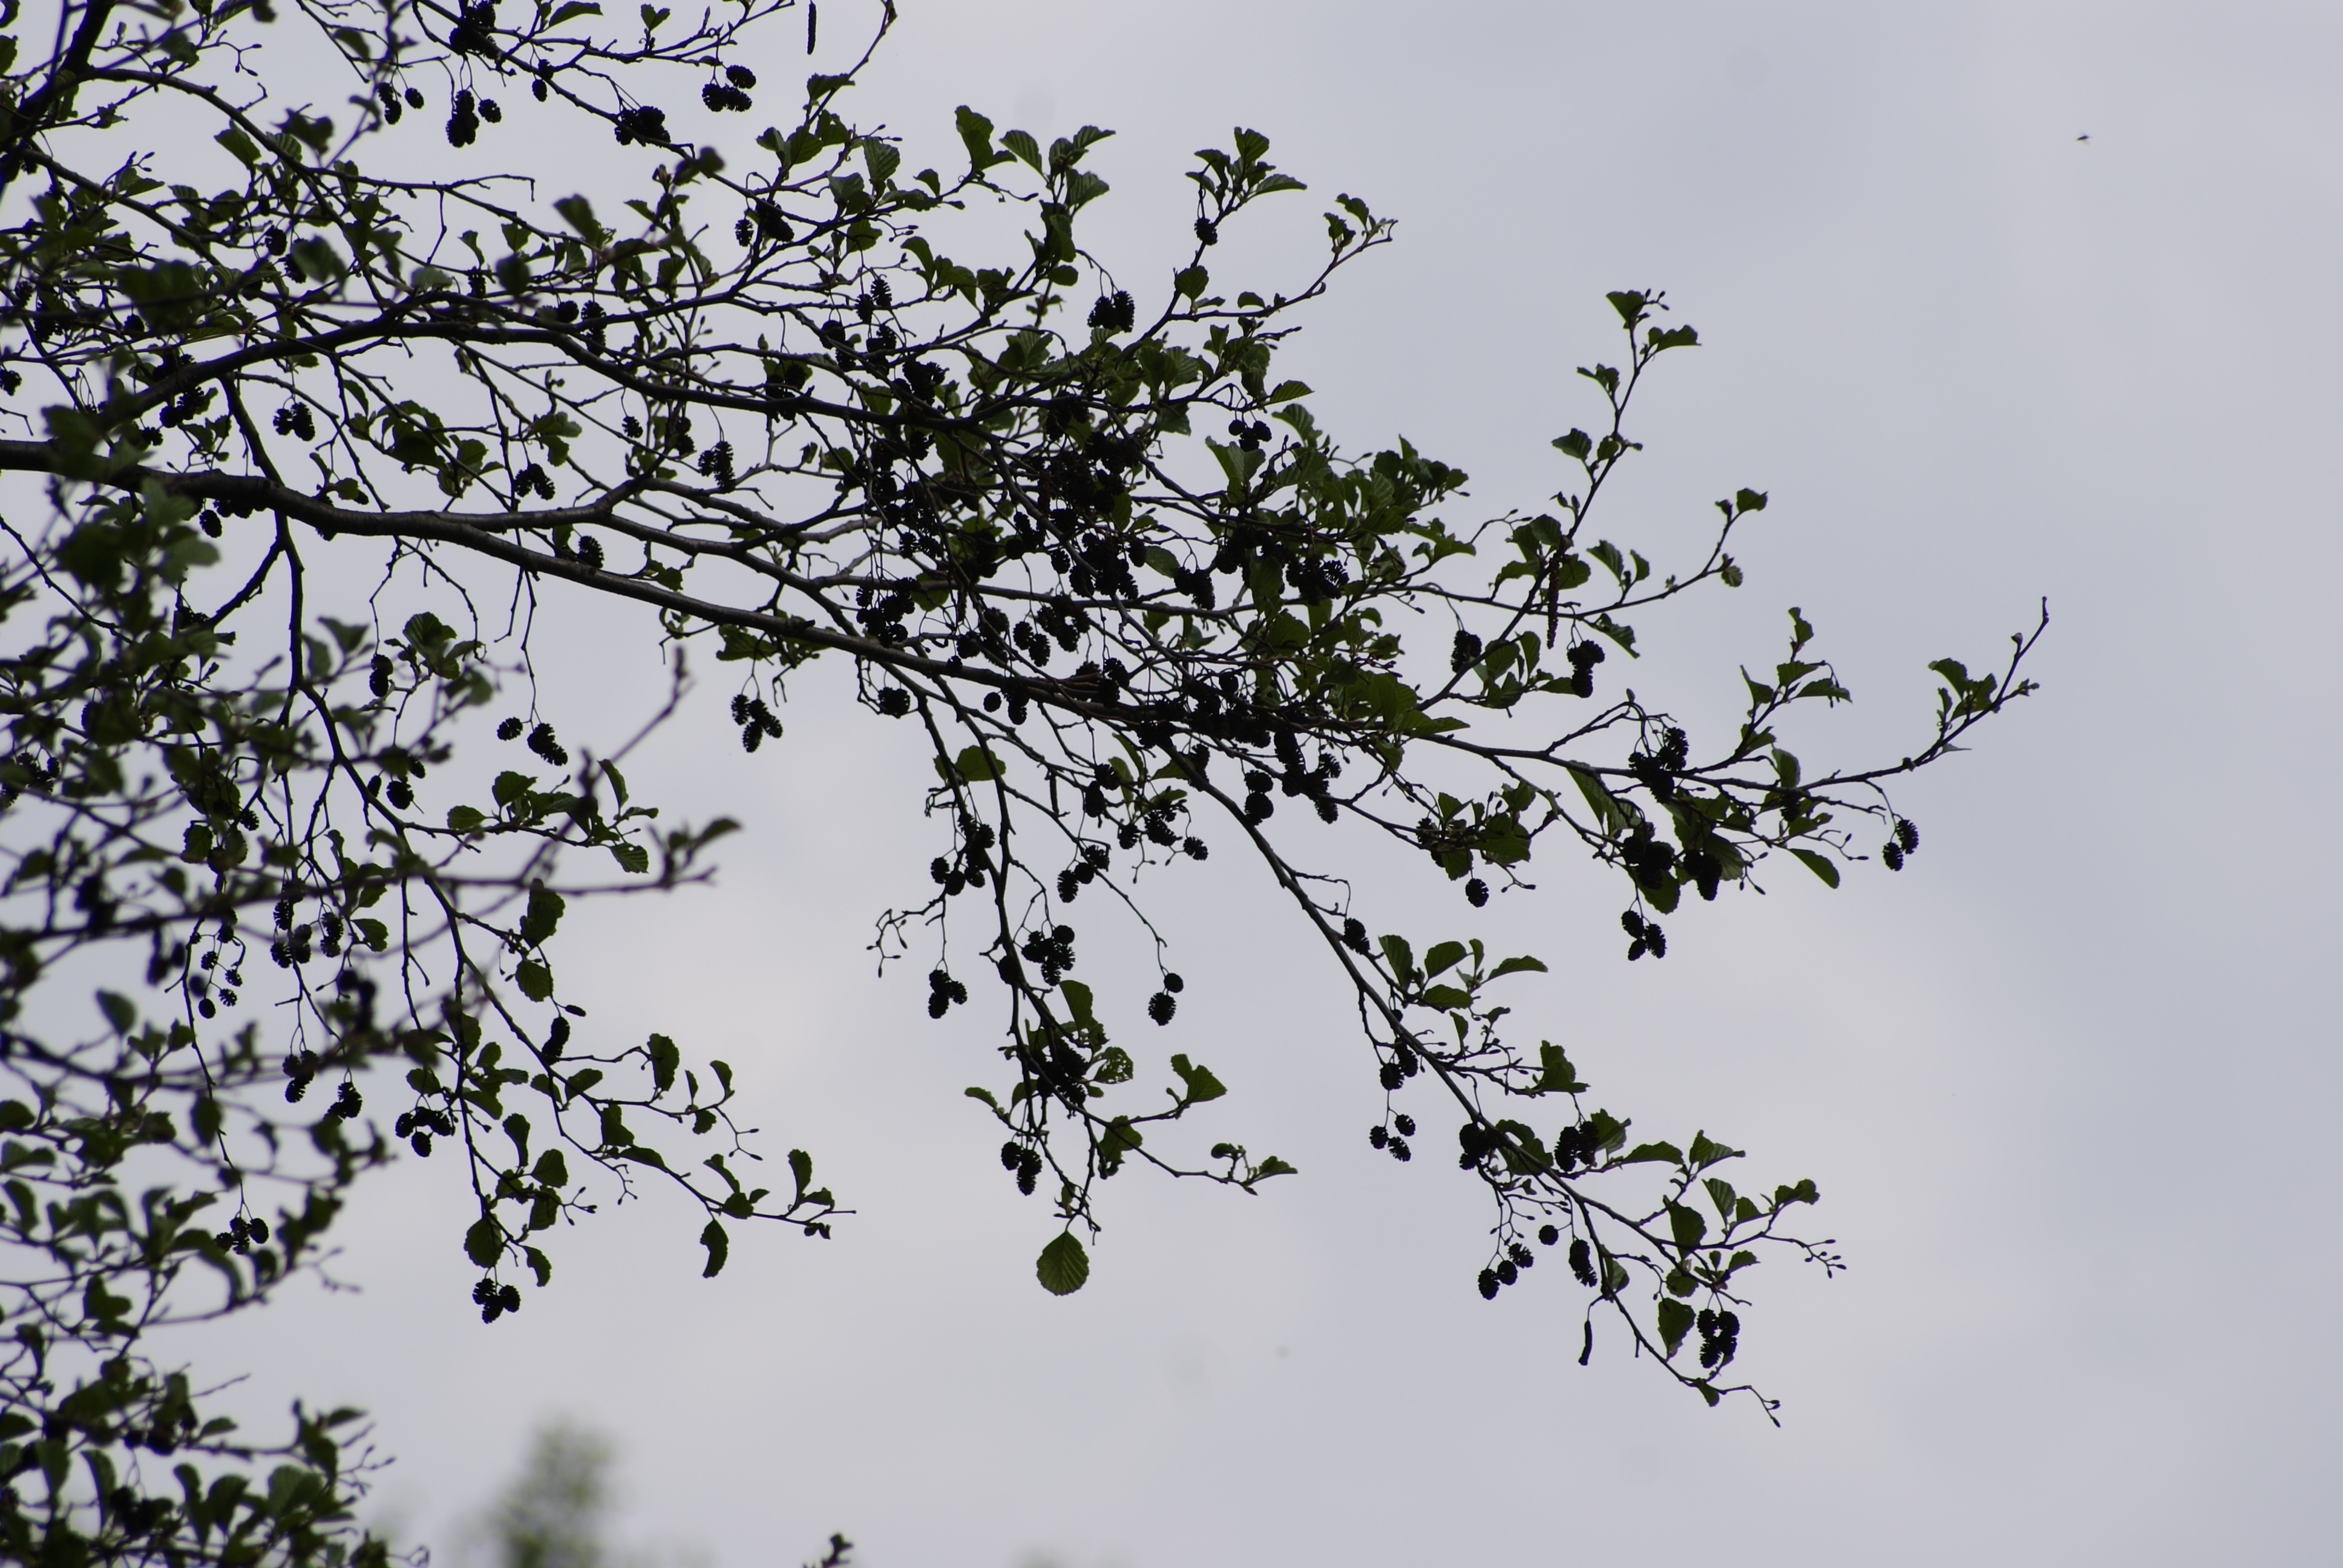
\includegraphics[width=90mm]{obr.jpg}
\caption{podpisisi}
\end{figure}

\chapter{Rozwiązanie - prezentacja wyników}

Zrealizowana aplikacja składa się z dwóch części, tj. aplikacji na androida oraz
serwera www. Serwer, czyli Servlet (aplet Javy) posiada połączenie z bazą
danych, w której przechowywane są informacje o przesyłce, kurierach i
klientach. Aplikacja mobilna również posiada połączenie z bazą danych, jednakże
połączenie to zrealizowano pośrednio. Aplikacja poprzez zapytania i odpowiedzi z
serwera uzyskuje informacje o stanie bazy danych. 

\begin{figure}[h]
\centering
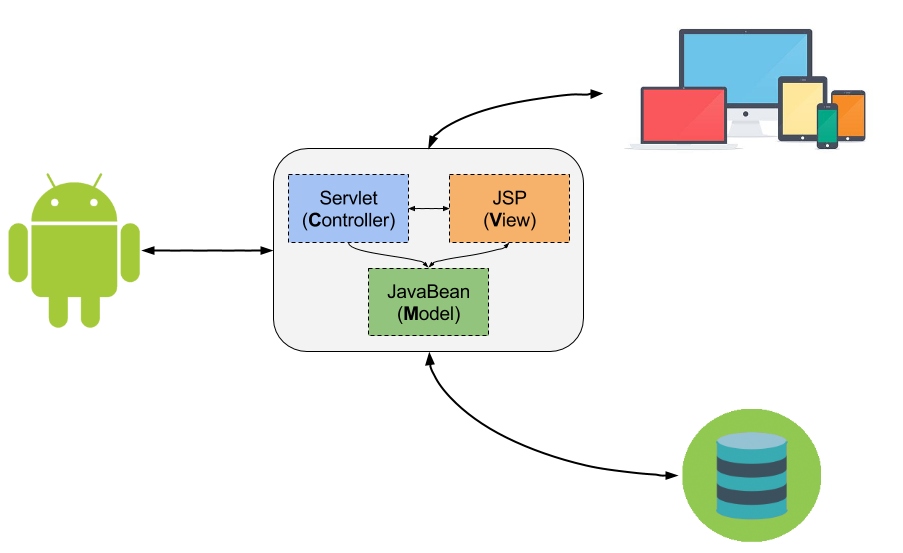
\includegraphics[width=100ex]{StrukturaSystemu.png}
\caption{Struktura systemu}
\label{StrukturaSystemu}
\end{figure}

Ideę systemu zaprezentowano na rysunku \ref{StrukturaSystemu}.
Aplikację zrealizowano w środowisku programistycznym Eclipse.

\emph{\color{komentarz} komentarz: dopisać pierdół wstępowych}

\newpage
\section{Aplikacja na system Android}

Założeniem aplikacji mobilnej było lokalizowanie kuriera i wysyłanie jego
pozycji na serwer, który zapisuje ją w bazie danych. Zasada działania aplikacji
polega na odpytaniu kuriera o jego numer id, a następnie sprawdzeniu czy jest
włączony GPS. Ponadto aplikacja wykrywa czy wprowadzono poprawne id oraz
zapobiega zalogowaniu się dwóch kurierów na tym samym id. Po wpisaniu poprawnego
id kuriera aplikacja zapamiętuje go i do automatycznie wysyła swoją pozycję.

\begin{wrapfigure}{r}{0.4\textwidth}
\centering
\captionsetup{justification=centering,margin=0cm}
\begin{center}
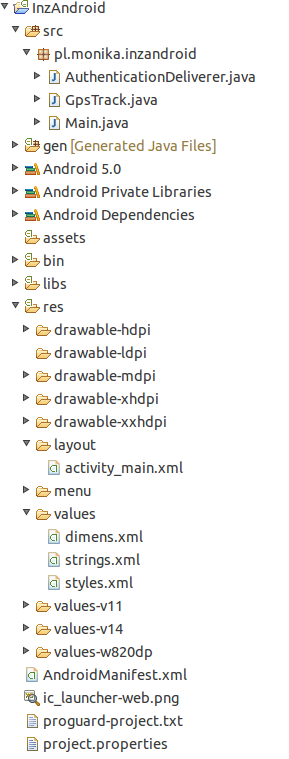
\includegraphics[width=.3\textwidth]{struktura_android.png}
\end{center}
\caption{Struktura programu aplikacji Android}
\label{fig:androidStruktura}
\end{wrapfigure}

Stworzenie aplikacji na system Android zostało rozpoczęte od doinstalowania
pluginu ADT (Android Development Kit) do programu Eclipse. Na ADT składają się
elementy Android SDK, gdzie SDK to Software Development Kit. Android SDK
zawiera w sobie takie elementy jak Tools - służy do tworzenia aplikacji niezależnie od
wersji systemu Android oraz Platform Tools - narzędzia stworzone pod kątem
wersji systemu Android. W skład SDK Tools wchodzą taki funkcje jak zarządzanie
projektami, modułami czy maszynami wirtualnymi, debugger, emulator. Natomiast
Platform Tools zawiera biblioteki do systemu Android. Plugin ADT  korzysta
z funkcji Android SDK i pomaga tworzyć, budować, instalować oraz debugować
aplikacje na system Android w środowisku Eclipse. W programie Eclipse tworzona
jest z aplikacją odpowiednia struktura projektu [rys. \ref{fig:androidStruktura}], w
której jest podział na klasy zawierające logikę aplikacji (scr), pliki generowane przez kompilator (gen),
folder na pliki z zasobami (assets), pliki binarne(bin), dodatkowe biblioteki
(libs) oraz folder na zasoby(res), którego odróżnia od assets to, że są
generowane do pliku R.java (nie trzeba podawać lokalizacji zasobów tylko jego
nazwę). W katalogu res również ustalana jest konfiguracja systemu - 
,,AndroidManifest.xml'', layout (wygląd i ustawienie elementów na ekranie
systemu Android), w podfolderach Drawable pliki graficzne, w podfolderach values
ciągi znaków(stringi, kolory) i ustawienia oraz w katalogu menu, w którym
ustawiane są dostępne opcje menu.

Projektowanie aplikacji Android zaczyna się od ustawienia layoutu aplikacji
(/res/layout/activity\_main.xml). Zaprojektowany przez autora layout jest
prosty i przejrzysty, ponieważ ma wykonywać bardzo podstawowe funkcje [rys.
\ref{fig:androidViewOK}]. I tak zawiera w sobie pole do wpisywania id kuriera,
pole wyświetlające komunikaty oraz przycisk wyłączający aplikację. Aplikacja została
tak przemyślana, że aby ją wyłączyć trzeba użyć przycisku ,,Off'', pozostałe hardware'owe przyciski
nie wyłączają aplikacji, jedynie ją minimalizują. Takie właściwości zostały
stworzone z myślą o tym, aby kurier podczas używania aplikacji tylko w świadomy
sposób mógł ją zamknąć.

Autor przewidział również odpowiednie zachowanie aplikacji, gdy kurier próbuje
zalogować się na nie istniejące w bazie id lub na id, które jest już zajęte -
tzn. na które już zalogował się inny kurier [rys. \ref{fig:androidViewNOTOK}]. 
Oprócz wyżej wymienionych zachowań aplikacji, w pasku statusu na telefonie
wyświetlana jest ikona podczas włączonej aplikacji a także w
powiadomieniach [rys. \ref{fig:androidViewtask}].

Kolejnym krokiem było nadanie odpowiednich uprawnień aplikacji, do tego służy
plik ,,AndroidManifest.xml''. Aplikacja zostały przyznane uprawnienia do
sprawdzania statusu sieci komórkowej oraz WiFi, sprawdzania statusu sygnału
GPS, a także do korzystania z wyżej wymienionych [listing \ref{lst:manifest}].

\lstset{language=XML,
 keywords=[0]{uses,permission},
 keywordstyle=[0]{\color{green!50!black}},
 stringstyle=\color{blue}
 }
\begin{lstlisting}[caption=Nadanie uprawnień aplikacji
Android w pliku AndroidManifest.xml,label=lst:manifest] 
<uses-permission android:name="android.permission.INTERNET" />
<uses-permission android:name="android.permission.ACCESS_NETWORK_STATE" />
<uses-permission android:name="android.permission.ACCESS_FINE_LOCATION" />
<uses-permission android:name="android.permission.ACCESS_WIFI_STATE" />
\end{lstlisting}

\begin{figure}
\centering
\subfigure[Główny ekran aplikacji, oczekuje na wprowadzenie id kuriera]{
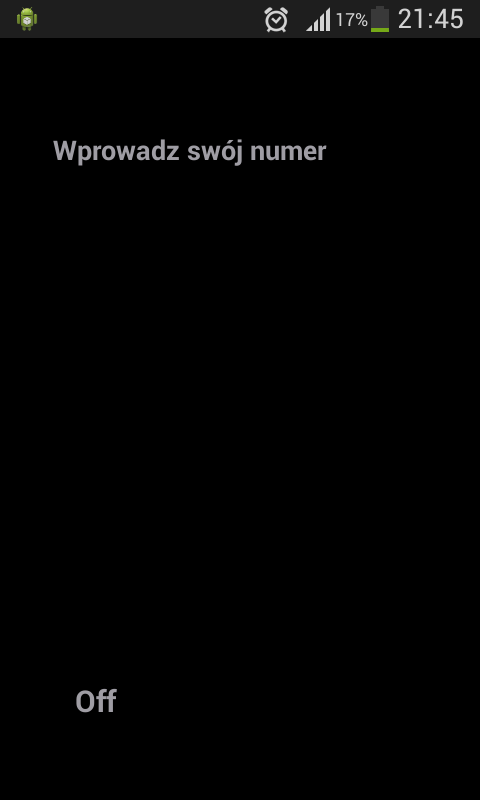
\includegraphics[height=0.33\textheight]{andWprowadz.png}
}
\subfigure[Gdy nie jest włączona sieć komórkowa lub WiFi na ekranie pokazuje
się komunikat i zostaje zablokowane pole do wprowadzania id]{
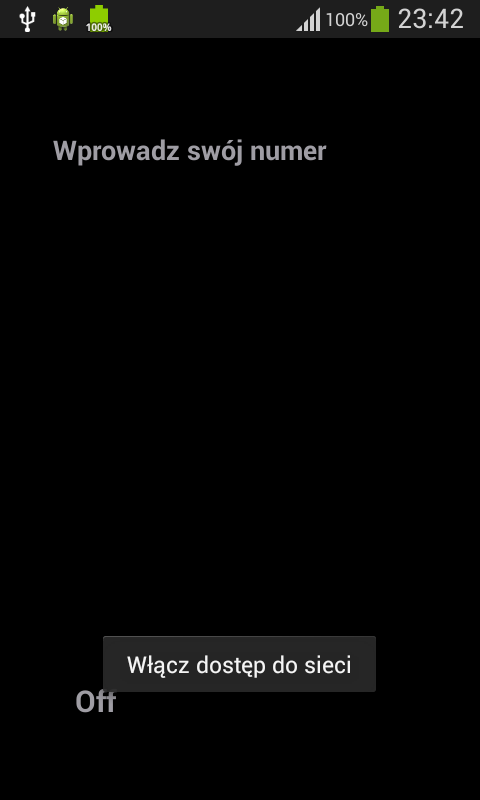
\includegraphics[height=0.33\textheight]{andWifi.png}
}
\subfigure[Komunikat o poprawnie wpisanym id]{
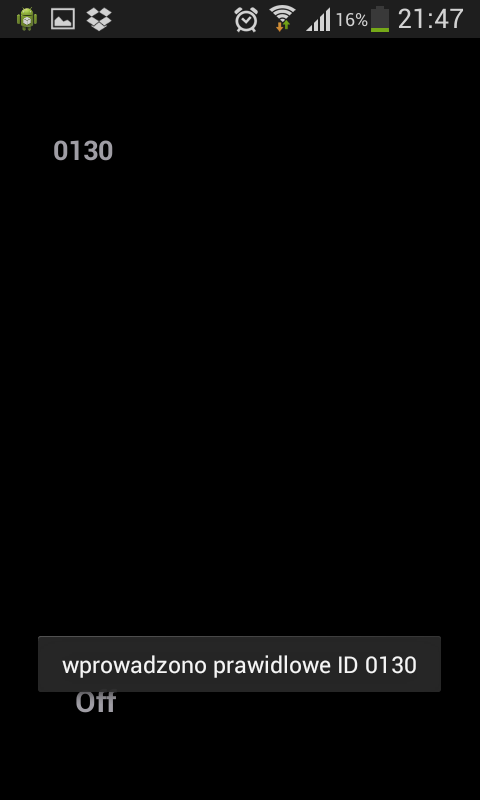
\includegraphics[height=0.33\textheight]{andID.png}
}
\subfigure[Informacje o niewłączonym GPS]{
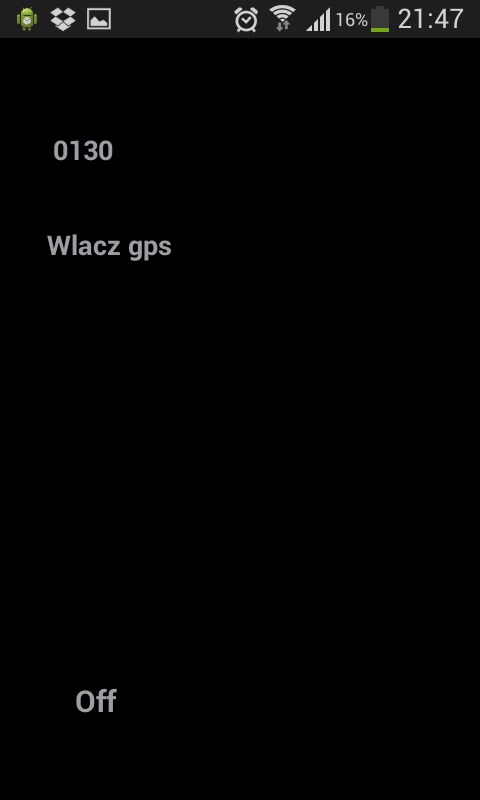
\includegraphics[height=0.33\textheight]{andGPS.png}
}
\subfigure[System czeka na ustalenie lokalizacji]{
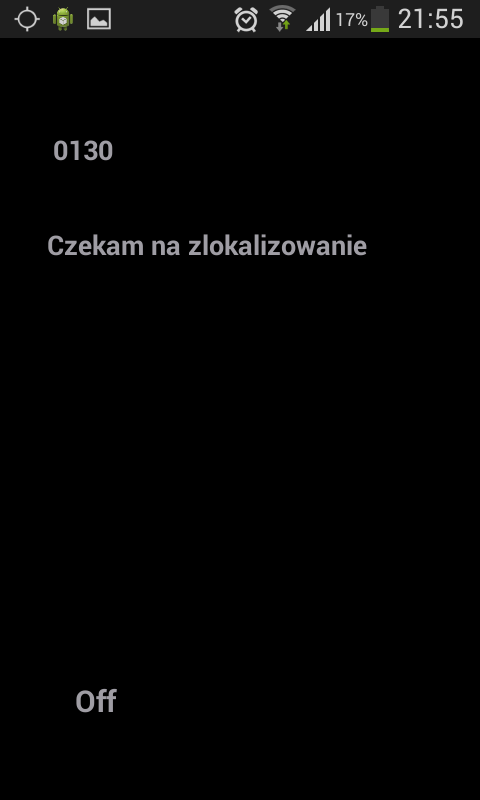
\includegraphics[height=0.33\textheight]{andCzeka.png}
}
\subfigure[System lokalizuje i wyświetla informacje o lokalizacji i czasie
odczytu]{
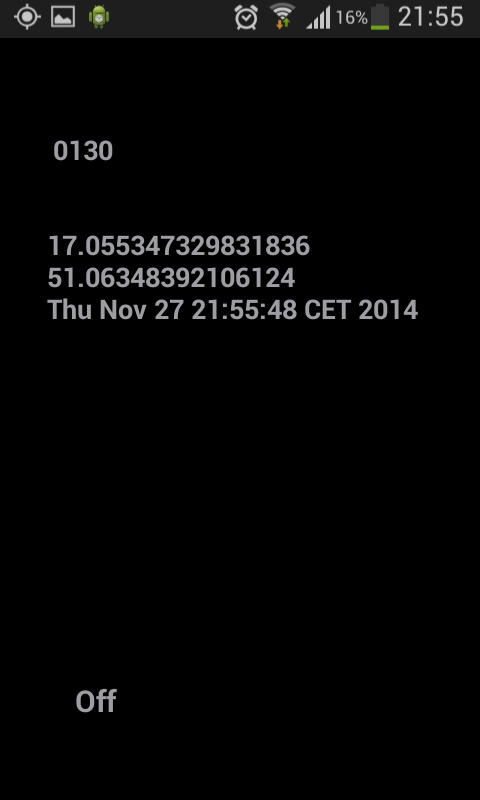
\includegraphics[height=0.33\textheight]{andLokal.png}
}
\caption{Ekrany Androida }
\label{fig:androidViewOK}
\vspace{-10pt}
\end{figure}

Po przygotowaniu wyglądu aplikacji oraz nadaniu jej uprawnień można przejść
do oprogramowania logiki aplikacji. Klasa główna, która zajmuje się obsługą
aplikacji dziedziczy po klasie \texttt{Activity}. Klasa \texttt{Ativity} zajmuje
się obsługą interakcji pomiędzy użytkownikiem a urządzeniem. Klasa ta tworzy okno aplikacji
oraz na przykład umieszcza ustawione wcześniej przyciski interfejsu użytkownika.
Znajdują się w niej takie metody jak \texttt{onCreate()}, \texttt{onDestroy()},
\texttt{onStart()}, \texttt{onStop()} i inne. Metodę \texttt{onCreate()} należy
przesłonić, jeśli mają być zainicjowane wcześniej wspomniane przyciski i pola z layoutu. Autor w swojej aplikacji nadaje
właściwość dla przycisku, która ma po kliknięciu go w dowolnym momencie
działania aplikacji wywołać zamknięcie aplikacji. Takie zachowanie osiąga się
poprzez wywołanie na rzecz niego metody \texttt{public void
setOnClickListener(View.OnClickListener l)}[listing \ref{lst:Main.button.java}].

\lstset{language=Java,firstnumber=1,stepnumber=1,keywords=[3]{button,savedId}}
\begin{lstlisting}[caption=Ustawienie właściwości przycisku
``Off'' w głównej klasie aplikacji mobilnej w
metodzie onCreate(),label=lst:Main.button.java] 

button.setOnClickListener(new View.OnClickListener() { 
	public void onClick(View v) { 
		if (savedId != "")
			new AuthenticationDeliverer().execute(savedId, "0", "0").get();
		savedId = "";
		onDestroy();
	}
});
\end{lstlisting}

Na listingu \ref{lst:Main.button.java} widać zmienną \texttt{savedId},
jest pole klasy, które zapisywane jest wpisanym przez kuriera jego \texttt{id}. Gdy użytkownik wyłącza
aplikację system sprawdza czy \texttt{savedId} nie jest puste i w przypadku gdy
\texttt{savedId} posiada jakąś wartość tworzony jest nowy obiekt
\texttt{AuthenticationDeliverer()} z odpowiednimi parametrami - nazwa
zmiennej, status aktywności oraz status logowania. Klasa
\texttt{AuthenticationDeliverer()} dziedziczy po \texttt{AsyncTask} (umożliwia
tworzenie nowego wątku i pozwala na wykonywanie operacji w tle). 

\begin{figure}[ht]
\centering
\captionsetup{justification=centering,margin=1cm}

\subfigure[sytuacja gdy jest już zajęte id lub nie istnieje]{
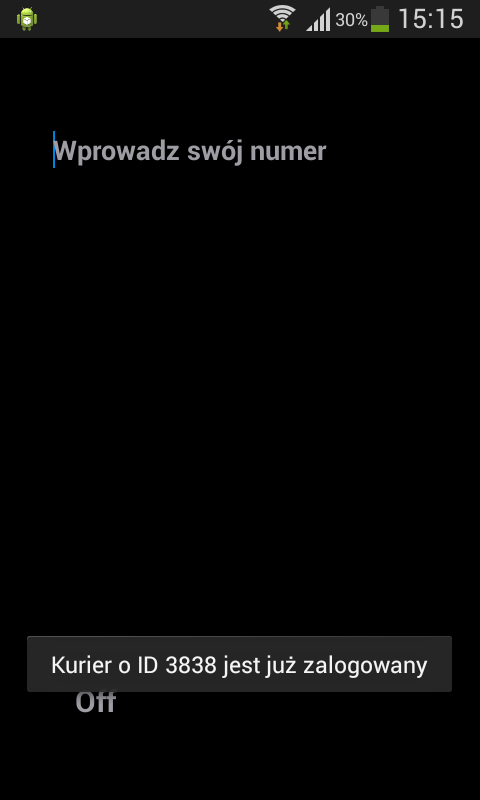
\includegraphics[width=25ex]{andJuzzalog.png}
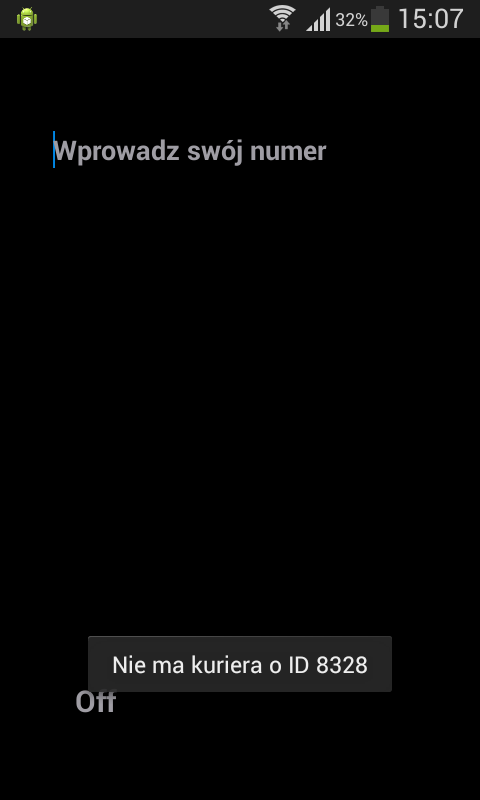
\includegraphics[width=25ex]{andNiema.png}
\label{fig:androidViewNOTOK}
}
\subfigure[status telefonu]{
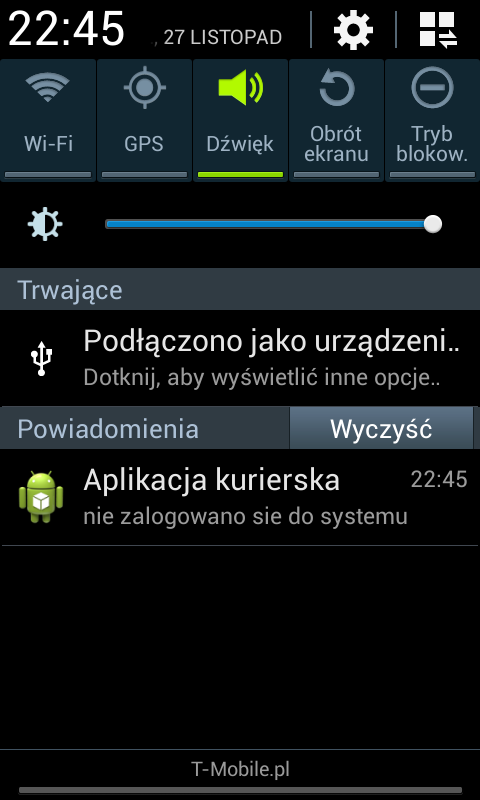
\includegraphics[width=25ex]{andBarNie.png}
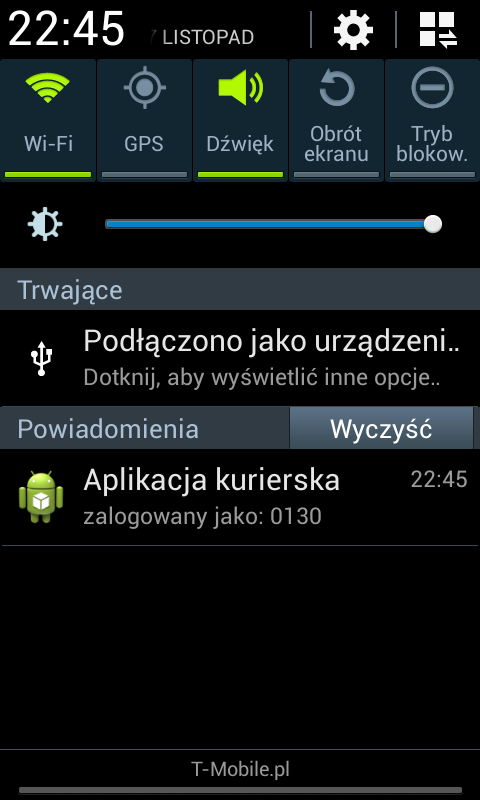
\includegraphics[width=25ex]{andBarZal.png}
\label{fig:androidViewtask}
}
\vspace{-10pt}
 \caption{Informacje o zalogowanym/nieistniejącym id i statusbar}
\vspace{-10pt}
\end{figure}

Parametry z jakimi tworzony jest
nowy obiekt to id kuriera, status aktywności oraz jego logowanie lub
wylogowywanie[listing. \ref{lst:AuthentictionDeliverer.java}]. Status aktywności to
informacja wysyłana do serwera (zapisywana w bazie danych) mówiąca o tym, czy kurier będzie ustawiał swój status na aktywny
czy nieaktywny - czy rozpoczyna pracę czy ją kończy. Status aktywności
sprawdzany jest ze statusem w bazie danych, jeśli kurier próbuje się zalogować,
ale w bazie jest już ktoś zalogowany na ten id pojawi się komunikat o
zalogowanym już kurierze o tym numerze [rys. \ref{fig:androidViewNOTOK}].
Natomiast trzeci parametr mówi o tym, czy kurier się zalogowuje ,,1'' czy wylogowuje ,,0''
z aplikacji. Na rzecz klasy AuthenticationDeliverer() wywołane zostają metody:
\texttt{execute()} - nakazuje wykonanie zadania, \texttt{get()} - oczekuje, aż
zadanie zostanie wykonane.

\lstset{language=Java,firstnumber=1,stepnumber=1,keywords=[3]{httpClient,localhost,httpPostAuthentication,httpGetAuthentication,httpResponse}}
\begin{lstlisting}[caption=klasa
AuthenticationDeliverer metoda
doInBackground,label=lst:AuthentictionDeliverer.java]
protected String doInBackground(String... params) {
	ArrayList<NameValuePair> pairs = new ArrayList<NameValuePair>();
	pairs.add(new BasicNameValuePair("ID", params[0]));
	pairs.add(new BasicNameValuePair("activ", params[1]));
	pairs.add(new BasicNameValuePair("logout", params[2]));
	httpPostAuthentication.setEntity(new UrlEncodedFormEntity(pairs));
	new Thread(new Runnable() {
		@Override
		public void run() {
				httpClient.execute(httpPostAuthentication);
		}
	}).start();
	httpResponse = (new DefaultHttpClient()).execute(httpGetAuthentication);
	String entityStr = EntityUtils.toString(httpResponse.getEntity());
	if (entityStr.contains("logIn"))
		return "logIn";
	else if (entityStr.contains("busy"))
		return "busy";
	else if (entityStr.contains("false"))
		return "false";
	else if (entityStr.contains("logOut"))
		return "logOut";
	return "";
}
\end{lstlisting}

Po zainicjalizowaniu pola edycji zostaje wywołana na rzecz niego metoda public
void addTextChangedListener(TextWatcher watcher), która oczekuje, aż w polu
tekstowym użytkownik wpisze odpowiedni ciąg znaków, systemowo dozwolone są
tylko cyfry.
W tym przypadku wykorzystano metodę abstract void afterTextChanged(Editable s) z interfejsu
TextWatcher. Po wpisaniu przez kuriera czterech cyfr następuje weryfikacja
wpisanego id. Po pozytywnym przejściu weryfikacji id kuriera aplikacja sprawdza
czy w urządzeniu jest włączony moduł GPS. Gdy spełnione zostaną wszystkie
warunki uruchamiany jest handler, który sczytuje pozycję kuriera i wysyła ją na
serwer wraz z datą, w której nastąpił odczyt. 

Odczyt pozycji GPS dostępny jest dzięki użyciu klasy LocationManager, która
zapewnia dostęp do lokalizacji systemu. LocationManager należy zainicjalizować
klasą Context (umożliwia dostęp do zasobów systemu i informację o nim),
natomiast getSystemService jest do kontroli pobierania lokalizacji. Następnie
ustawiono z jaką częstotliwością ma być odczytywana zmiana pozycji. Po wykonaniu
tych czynność następuje zapytanie o ostatnią znaną pozycję. Całą
procedurę odczytu pozycji GPS pokazano na listingu \ref{lst:GpsTrack.java}.

\lstset{language=Java,firstnumber=31,stepnumber=1,keywords=[3]{locationManager,context,minTime,minDistance,location,longitude,latitude}}
\begin{lstlisting}[caption=Pobieranie lokalizacji
kuriera metoda getLocation() z klasy GpsTrack,label=lst:GpsTrack.java]

public Location getLocation() {
	locationManager = (LocationManager) context
			.getSystemService(Context.LOCATION_SERVICE);
	locationManager.requestLocationUpdates(LocationManager.GPS_PROVIDER,
			minTime, minDistance, (android.location.LocationListener) this);
	if (locationManager != null) {
		location = locationManager.getLastKnownLocation(LocationManager.GPS_PROVIDER);
		if (location != null) {
			longitude = location.getLongitude();
			latitude = location.getLatitude();
		}
	}
	return location;
}
\end{lstlisting}

Ostatnią istotną częścią jaka realizowana jest na systemie Android to połączenie
z serwerem. Nim zostanie nawiązane połączenie konieczne jest przygotowanie
treści wiadomości jaka ma zostać wysłana na adres serwer. Następuje to poprzez
wpisanie par ciągów znaków, w tym jedna część to identyfikator, a druga to jego
wartość, do tablicy. Na jej podstawie wystosowany jest URL httpPost i wykonywany
na kliencie http (tutaj na Servlecie). Taka wiadomość może wyglądać w tym
przypadku tak:
\begin{flushright}
\texttt{http://192.168.1.2:8080/inzServlet/insert?ID=0130\&longitude=50.3545\&latitude=11.3483
\\$\hookrightarrow$\&timestamp=2014-11-25+15:14:55\&activ=1}
\end{flushright}

\lstset{language=Java,firstnumber=1,stepnumber=1,keywords=[3]{savedId,
httpClient, httpPost,localhost}}
\begin{lstlisting}[caption=Metoda startSendGpsDate() klasy
main.java. Metoda sprawdza stan sygnału GPS i przygotowuje wiadomość do
wysłania na serwer oraz wysyła ją,label=lst:Main.startSendGpsDate.java]
private String localhost = "192.168.1.2:8080";
private HttpClient httpClient = new DefaultHttpClient();
private HttpPost httpPost = new HttpPost("http://" + localhost
		+ "/inzServlet/insert");
(*@\centerline{\raisebox{0pt}[0pt][0pt]{$\vdots$}}@*)
private void startSendGpsDate() {
	if (gpsTrack.isGpsEnable()) {
		gpsTrack.getLocation();
		double lat = gpsTrack.getLatitude();
		double lon = gpsTrack.getLongitude();
		if (lat != 0.0 && lon != 0.0) {
			Date date = new Date(System.currentTimeMillis());
			textView.setText(lon + "\n" + lat + "\n" + date);
			ArrayList<NameValuePair> pairs = new ArrayList<NameValuePair>();
			pairs.add(new BasicNameValuePair("ID", savedId));
			pairs.add(new BasicNameValuePair("longitude", lon + ""));
			pairs.add(new BasicNameValuePair("latitude", lat + ""));
			pairs.add(new BasicNameValuePair("timestamp",
					new SimpleDateFormat("yyyy-MM-dd HH:mm:ss").format(date)));
			pairs.add(new BasicNameValuePair("activ", 1 + ""));
			httpPost.setEntity(new UrlEncodedFormEntity(pairs));
			new Thread(new Runnable() {
				@Override
				public void run() {
					httpClient.execute(httpPost);
				}
			}).start();
		} else
			textView.setText("Czekam na zlokalizowanie");
	} else {
		textView.setText("Wlacz gps");
	}
}
\end{lstlisting}

W powyższym paragrafie zostały opisane kluczowe funkcje klas zaimplementowanych
na systemie Android. W opisie i w listingach ominięto obsługę wyjątków. 

\section{Serwer}

W niniejszej pracy skorzystano możliwości rozszerzenie języka Java o funkcje
serwera WWW. Przez takie wykorzystanie języka Java takie serwer nazywany jest
wtedy Serwletem - aplet Javy. Zadaniem serwera było obsłużenie klientów firmy
kurierskiej, którzy wpisując numer swojej przesyłki mogli sprawdzić gdzie ona
się aktualnie znajduje. Oprócz tej funkcji Servlet też jest pośrednikiem
między aplikacją mobilną a bazą danych.

\begin{wrapfigure}{r}{0.4\textwidth}
\centering
\captionsetup{justification=centering,margin=0cm}
\vspace{-10pt}
\begin{center}
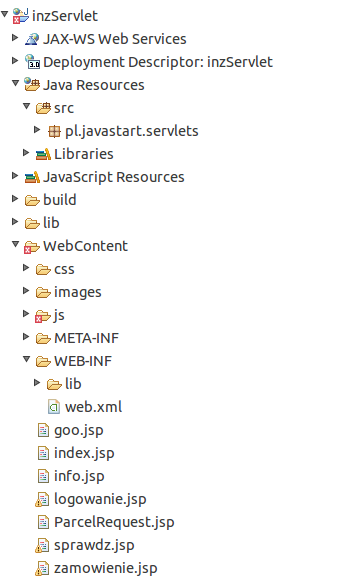
\includegraphics[width=.35\textwidth]{strukturaServlet.png}
\end{center}
\vspace{-10pt}
  \caption{Struktura plików Servletu}
\label{fig:servlet}
\vspace{-60pt}
\end{wrapfigure}

Rozpoczęcie pracy z servletem wymagało zainstalowanie dodatków do środowiska
Eclipse:
\begin{itemize}
  \item Eclipse Java EE Developer Tools
  \item Eclipse Java Web Developer Tools
  \item Eclipse Web Developer Tools
  \item JST Server Adapters
  \item JST Server Adapters Extensions
\end{itemize}

Po zainstalowaniu dodatków należało skonfigurować środowisko, w tym celu należało
stworzyć nowy lokalny serwer. Autor skorzystał z popularnego serwera Apache
Tomcat wersji 7.0. Serwer jest dostępny pod adresem localhost:8080. 

Po skonfigurowaniu środowiska można było przystąpić do utworzenia nowego
dynamicznego projektu sieciowego (\textsl{Dynamic Web Project}). W strukturze
projektu najważniejsze są dwa foldery [rys.\ref{fig:servlet}], jeden zawierający
w sobie klasy Javy, drugi zawierający obsługę, wygląd stron Servletu. W tymże
folderze znajduje się plik ,,web.xml'', w którym definiuje zachowanie serwera w
zależności od tego jaki adres został wpisany w przeglądarkę. 

Na poniższym listingu widać ustawienie strony startowej
(\texttt{<welcome-file-list>}), tzn. gdy w polu adresy wpisany jest
http://localhost:8080/inzServlet uruchamia się strona główna aplikacji webowej -
Index.jsp. W następnej liniach jest załadowanie klasy
Javy(\texttt{pl.javastart.servlets.Sprawdz}) do Servletu pod nazwą
\texttt{Sprawdz} i zmapowanie tej klasy pod adres
http://localhost:8080/inzServlet/sprawdz. Pokazany tu sposób dotyczy wszystkich
używanych przez Servlet klas Javy, w podobny sposób można zadeklarować użycie
pliku *.jsp (różnica polega na zamianie identyfikatora \texttt{<servlet-class>}
na \texttt{<jsp-file>}). 

\lstset{language=XML,firstnumber=1,stepnumber=1}
\begin{lstlisting}[caption=Fragment pliku web.xml,label=lst:web.xml]
<welcome-file-list>
	<welcome-file>index.jsp</welcome-file>
</welcome-file-list>
<servlet>
	<servlet-name>Sprawdz</servlet-name>
	<servlet-class>pl.javastart.servlets.Sprawdz</servlet-class>
</servlet>
<servlet-mapping>
	<servlet-name>Sprawdz</servlet-name>
	<url-pattern>/sprawdz</url-pattern>
</servlet-mapping>
<servlet>
	<servlet-name>Index</servlet-name>
	<jsp-file>/index.jsp</jsp-file>
</servlet>
<servlet-mapping>
	<servlet-name>Index</servlet-name>
	<url-pattern>/index</url-pattern>
</servlet-mapping>
\end{lstlisting}

Każda klasa Javy, która rozszerza Servlet posiada dwie istotne metody do obsługi
stron serwera - \texttt{doPost} i \texttt{doGet}, obydwie przyjmuję argument
typu \texttt{HttpServletRequest} i \texttt{HttpServletResponse}.
Metody mają zapewniać komunikację pomiędzy serwerem a klientem. Argument
\texttt{HttpServletRequest} zawiera żądanie klienta do wykonania na serwlecie,
natomiast \texttt{HttpServletResponse} jest odpowiedziom serwera na żądanie
klienta.
Wspomniana metoda \texttt{doGet} obsługuje żądania jakie powstały w nagłówku http - pobiera
parametry i przetwarza je - obsługuje zadania typu request. Metoda doPost
również obsługuje żądanie powstałe z uzupełnienia formularzy. 

Ważną klasą w projekcie jest klasa obsługująca bazę danych. Klasa do obsługi
bazy danych musi składać się z następujących poleceń: załadowanie sterownika
bazy danych, nawiązanie połączenia z bazą, pobranie/zapisanie danych, zamknięcie
połączenia. Przykładem obsługi bazy danych jest poniższy listing [listing
\ref{lst:CheckIsExistsDeveliverer.selectFromDB.java}]. Przedstawiona metoda sprawdza czy istnieje w
bazie dany kurier. Sprawdzenie istnienia kuriera realizowane jest przez
zapytanie \texttt{"select * from deli.deliverer where id=" + id}, gdzie id jest
identyfikatorem kuriera. Po wykonaniu zapytania pod \texttt{ResultSet}
zapisywane są dane pobrane z bazy danych, z nich wyszukiwane są potrzebne informacje, czyli
id kuriera oraz jego status aktywności. \texttt{Id} pobierane jest tylko w celu
sprawdzenia czy w bazie istnieje kurier, niestety nie ma metody dla
\texttt{ResultSet} która sprawdzałaby czy wynik zapytania jest pusty. Po
uzyskaniu wyniku, że kurier istnieje sprawdzana jest jego aktywność, gdy kurier
jest nie aktywny a funkcja była wywoływana w celu zalogowania systemu
przygotowywane jest zapytanie o zaktualizowanie danych dla tego kuriera i
ustawieniu jego aktywności na stan aktywny (\texttt{true}). Natomiast gdy
aktywność id kuriera jest \texttt{true}, a kurier pragnie się zalogować (metoda została
wykonana dla zalogowania do systemu) metoda zwraca ciąg ,,busy'' - informuje o zajętości id.
W momencie wylogowywania kuriera (kiedy aktywność == \texttt{true}) a
\texttt{logout} wynosi 0 to przygotowywana jest komenda aktualizująca bazę
danych i pod wskazaną krotkę o numerze id zapisywana wartość 0 dla activ.

\lstset{language=Java,firstnumber=1,stepnumber=1,keywords=[3]{id,activ,logout}}
\begin{lstlisting}[caption=Połączenia z bazą danych na przykładzie metody
sprawdzającej istnienie kuriera oraz jego stan
używanej przez aplikację
mobilną,label=lst:CheckIsExistsDeveliverer.selectFromDB.java]
Class.forName("com.mysql.jdbc.Driver");
Connection connection = DriverManager.getConnection(
		"jdbc:mysql://localhost:3306/deli", "root", "sun5flower");
Statement statement = connection.createStatement();
stringSelect = "select * from deli.deliverer where id=" + id;
ResultSet resultSet = statement.executeQuery(stringSelect);

while (resultSet.next()) {
	delivererId = resultSet.getInt("id");
	delivererActiv = resultSet.getBoolean("activ");
} 
if (delivererId > 0) {
	if (delivererActiv == false) {
		sqlInsert = " update deli.deliverer set activ=1 where id=" + id;
		statement.executeUpdate(sqlInsert);
		connection.close();
		statement.close();
		return "logIn";
	} else if (delivererActiv == true) {
		if (logout.equals("0")) {
			sqlInsert = " update deli.deliverer set activ=0 where id=" + id;
			statement.executeUpdate(sqlInsert);
			connection.close();
			statement.close();
			return "logOut";
		} else if (logout.equals("1")) {
			connection.close();
			statement.close();
			return "busy";
		}
	}
} else
	return "false";
\end{lstlisting}

Projekt dążył do stworzenia przyjaznego dla użytkownika-klienta widoku
lokalizacji przesyłki. Do osiągnięcia tego celu użyto zmodyfikowanego przez
autora darmowego szablonu pobranego z internetu \cite{szablon}. W zakładce
\texttt{SPRAWDZ PRZESYLKE} wpisywany jest numer przesyłki jaką klient chce
sprawdzić [rys.
\ref{fig:sprawdz}]. Wpisany ciąg znaków jest sprawdzany pod kątem poprawności.
Sprawdzane jest czy ciąg w formularzu jest liczbowy i czy istnieje taka
przesyłka. Gdy w bazie nie istnieje przesyłka pojawia się odpowiedni komunikat
informujący o nie istniejącej przesyłce [rys. \ref{fig:niema}]. Gdy użytkownik
wprowadzi poprawny numer przesyłki zostaną wyświetlone takie informacje, jak
nadawca, odbiorca, czas nadania i czas odbioru oraz ostanie sczytane położenie
przesyłki. Ponadto wyświetlana jest mapa pokazująca jak trasę pokona przesyłka -
znaczniki A - B. Na mapie dodatkowo pokazany jest znacznik, który wyznacza
pozycję kuriera z daną przesyłką - znacznik ,,kurier''.

Istotną częścią projektu było zaprojektowanie strony, na której
klient może sprawdzać status swojej przesyłki zrealizowane jest to poprzez utworzenie pliku
*.jsp, i przypisanie jej adresu http. Ogólny zarys pliku sprawdz.jsp jest
pobrany z szablonu \cite{szablon}, autor zmienił jedynie ciało (main) pliku. 

\begin{figure}[ht!]
\centering

\includegraphics[width=\textwidth]{sprawdz.png}
\caption{Widok strony internetowej\texttt{SPRAWDZ} serwisu z zachętą do
wprowadzenia numeru przesyłki do sprawdzeni}
\label{fig:sprawdz}
\end{figure}

\begin{figure}[ht!]
\centering
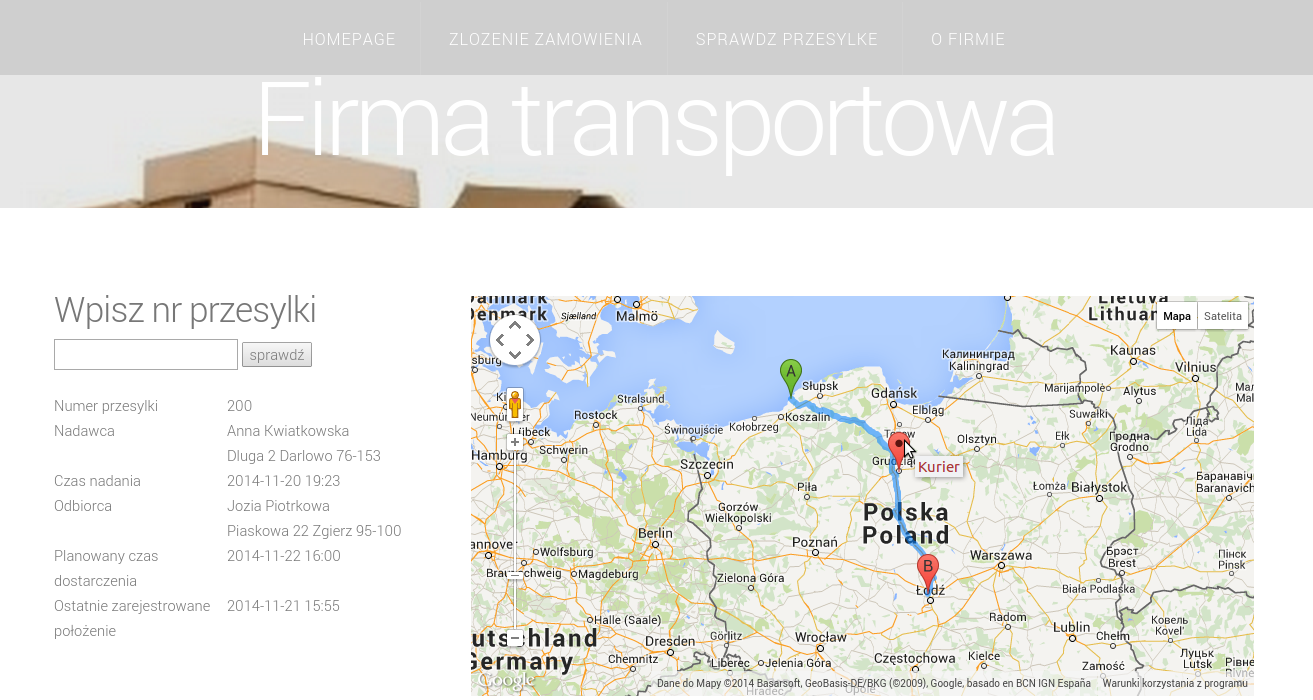
\includegraphics[width=\textwidth]{przyklad.png}
\caption{Widok strony internetowej \texttt{SPRAWDZ} z wyznaczoną trasą dla
przykładowej przesylki}
\label{fig:pokaz}
\end{figure}

\begin{figure}[ht!]
\centering

\includegraphics[width=\textwidth]{nieMaPrzesylki.png}
\caption{Przykład odpowiedzi serwisu na nieprawidłowe wpisanie numeru przesyłki}
\label{fig:niema}
\end{figure}


Z formularza [rys. \ref{fig:sprawdz}] pobierany jest numer poszukiwanej
przesyłki [listing \ref{lst:sprawdz.jsp} linie
\ref{lst:sprawdz.jsp1}-\ref{lst:sprawdz.jsp2}] i ustawiany jako post formularza i przesyłany do klasy Java Servletu. W tej klasie po
pobraniu danych z bazy danych zwracane są wartości dotyczące istnienia przesyłki
o wskazanym id. Najpierw sprawdzane jest, we fragmencie kodu Javy w instrukcji
warunkowej, czy przesyłka istnieje \texttt{isParcelExists}. Gdy przesyłka
nie zostanie odnaleziona w bazie lub wpisany ciąg w formularzu jest niepoprawny
wyświetlana jest wiadomość [listing \ref{lst:sprawdz.jsp} linia
\ref{lst:sprawdz.jsp6}] dotycząca błędnego id. Natomiast gdy wpisany id jest
bezbłędne w tabeli [rys.
\ref{fig:pokaz}] zostają wypisane dane dotyczące przesyłki oraz mapa. Linia
\ref{lst:sprawdz.jsp5} listingu \ref{lst:Sprawdz.jsp} jest miejscem użycia
JavySciprt'owego kodu google.maps. W danych wejściowych zmienna msg oznacza wiadomość dotyczącą
niepoprawnie wpisanego numeru przesyłki lub jeśli przesyłka została poprawnie
wpisana, ale jej ostatnie położenie jest zarejestrowane w centrali to w tabeli
w wierszu ,,Ostatnie zarejestrowane położenie'' pojawia się dodatkowa informacje
o przebywaniu przesyłki w centrali.

\emph{\color{komentarz}komentarz: zrobić tu jakaś przeorganizowanie, żeby nie
było tak że zdjęcie obok listingu}

\lstset{language=Java,firstnumber=1,stepnumber=1,keywords=[4]{script,
div,section,
table,td,tr,h2,form,input,br},keywords=[5]{width,id,method,action,type,name,value,style}}
\begin{lstlisting}[caption=Ciało pliku JavaServlet Pages -
sprawdz.jsp,label=lst:Sprawdz.jsp] 
(*@\label{lst:sprawdz.jsp1}@*)<h2>Wpisz nr przesylki</h2> 
	<form id="formularz" method="post" action=""> 
	<input type="text" name="nr" /> <input type="submit" value="sprawdz" />
</form> (*@\label{lst:sprawdz.jsp2}@*)
(*@\hspace{4ex}{\raisebox{-1pt}[0pt][0pt]{$\vdots$}}@*)
(*@\label{lst:sprawdz.jsp3}@*)<%
if (request.getAttribute("isParcelExists") != null &&
request.getAttribute("isParcelExists").equals(true)) {
%>
(*@\label{lst:sprawdz.jsp4}@*)<table style="width:100%">
	<tr>
		<td><% out.print("Numer przesylki"); %></td>
		<td>${id}</td>
	</tr>
	<tr>
		<td><% out.print("Nadawca"); %></td>
		<td>${regUserName}<br> ${regUserAddr} </td>
	</tr>
	<tr>
		<td><% out.print("Czas nadania"); %></td>
		<td>${timeSend}</td>
	</tr>
	<tr>
		<td><% out.print("Odbiorca"); %></td>
		<td>${userName}<br> ${userAddr} </td>
	</tr>
	<tr>
		<td><% out.print("Planowany czas"); %><br> <% out.print("dostarczenia"); %>
		</td>
		<td>${timeDelivery}</td>
	</tr>
	<tr>
		<td><% out.print("Ostatnie zarejestrowane"); %><br>
			<% out.print("polozenie"); %></td>
		<td>${lastTime}<br>${msg}</td>
	</tr>
</table>
(*@\hspace{4ex}{\raisebox{-1pt}[0pt][0pt]{$\vdots$}}@*)
(*@\label{lst:sprawdz.jsp5}@*)<div id="mapka"> </div>
(*@\hspace{4ex}{\raisebox{-1pt}[0pt][0pt]{$\vdots$}}@*)
<%
}
(*@\label{lst:sprawdz.jsp6}@*)else {
%>
(*@\label{lst:sprawdz.jsp7}@*)<br> ${msg} ${id}
<% 
}
%>
\end{lstlisting}

Natomiast ustawianie parametrów umieszczonych w \$\{\ldots\} zrealizowano
poprzez klasę rozszerzającą Servlet. Na listingu \ref{lst:Sprawdz.doPost.java}
przedstawiono metodę \texttt{doPost()} klasy \texttt{Sprawdz.java}, która odpowiada za uzupełnianie
pliku JSP \texttt{sprawdz.jsp} danymi dotyczącymi przesyłki, które są
wyświetlane w widoku strony dla klienta. Klasa \texttt{Sprawdz} tworzy nowy
obiekt klasy \texttt{SearchParcel} wywołując ją z argumentem id przesyłki.
Obiekt klasy \texttt{Searchparcel} odczytuje bazę danych i przypisuje
wartości zmiennym (listing \ref{lst:SearchParcel.selectFromDB.java}). Następnie sprawdzane
jest w instrukcji warunkowej if czy taka przesyłka istnieje i wprowadzone znaki są
typu integer, jeśli nie istniej to w zależności od tego jaki błąd wystąpił
przygotowywana jest wiadomość zwrotna dotycząca błędu. Natomiast jeśli przesyłka
istnieje ustawiane są parametry zwrotne
\texttt{req.setAttribute(``\ldots'',\ldots)}. Warto zwrócić uwagę na to, że
pierwszy argument \texttt{setAttribute} musi być zgodny z oczekiwaną nazwą
zmiennej w pliku JSP, w inny wypadku nie zostanie przypisana wartość z klasy
Javy do JSP. Na przykład argumenty z listingu \ref{lst:sprawdz.jsp} z linii
\ref{lst:sprawdz.jsp7} muszą się zgadzać argument z listingu
\ref{lst:Sprawdz.doPost.java} z linii \ref{lst:Sprawdz.doPost.java1}-\ref{lst:Sprawdz.doPost.java2}.

\lstset{language=Java,firstnumber=1,stepnumber=1,keywords=[3]{}} 
\begin{lstlisting}[caption=Fragment klasy Sprawdz.Java\,
metoda doPost(),label=lst:Sprawdz.doPost.java]
protected void doPost(HttpServletRequest req, HttpServletResponse resp) {
	String id = req.getParameter("nr");
	boolean isParcelExists = false;
	RequestDispatcher view = req.getRequestDispatcher("/sprawdz.jsp");
	if (id != null && (Sth.isInteger(id)) == true) {
		SearchParcel searchParcel = new SearchParcel(Integer.parseInt(id));
		if (searchParcel.getIsParcelExists() == true) {
			isParcelExists = true;
			req.setAttribute("id", id);
			req.setAttribute("lat", searchParcel.getDelivererLatitude());
			req.setAttribute("lon", searchParcel.getDelivererLongitude());
			req.setAttribute("regUserName",	searchParcel.getRegisteredUserNameUser());
			req.setAttribute("regUserAddr",	searchParcel.getRegisteredUserStreetUser() +
					" " + searchParcel.getRegisteredUserCityUser() + " " +
			searchParcel.getRegisteredUserCityCodeUser()); 
			req.setAttribute("timeSend", searchParcel.getParcelSendTime().substring(0, 16));
			req.setAttribute("userName", searchParcel.getParcelAddresseeName());
			req.setAttribute("userAddr", searchParcel.getParcelAddresseeStreet() + " " +
					searchParcel.getParcelAddresseeCity() + " "	+ 
					searchParcel.getParcelAddresseeCityCode());
			req.setAttribute("timeDelivery", searchParcel .getParcelDeliveryTime()
					.substring(0, 16)); 
			req.setAttribute("lastTime", searchParcel.getParcelTimePos().substring(0, 16));
			if (searchParcel.getDelivererId() > 999000) {
				searchParcel.selectBase(searchParcel.getDelivererId());
				req.setAttribute("msg", "Przesylka w bazie: "
						+ searchParcel.getCentreNameCentre());
			}
		} else {
			(*@\label{lst:Sprawdz.doPost.java1}@*)req.setAttribute("msg", "Nie mamy
			przesylki w bazie o numerze: ");
			(*@\label{lst:Sprawdz.doPost.java2}@*)req.setAttribute("id", id); 
	}
	if (id == null || (Sth.isInteger(id)) == false)
		req.setAttribute("msg", "Prosze podac poprawny numer przesylki"); 
	req.setAttribute("isParcelExists", isParcelExists);
	req.removeAttribute("nr");
	view.forward(req, resp);
};
\end{lstlisting}

Na podstawie źródła \cite{developer.google.maps} autor utworzył kod,
który wyświetla mapę ze znacznikami - markerami. Z danych metody post pobierane
są wartości lat i lon (szerokość i długość geograficzna) dla kuriera oraz wartości
\texttt{regUserAddr} i \texttt{userAddr} oznaczające adres nadawcy i odbiorcy. W
skrypcie tworzony jest nowy obiekt klasy DirectionsRenderer, który jest odpowiedzialny
wypełnienie(renderowanie) wyświetlanej mapy oraz tworzony jest nowy obiekt
\texttt{DirectionsService}, który jest wylicza trasę pomiędzy punktami.
Do obiektu \texttt{DirectionsRenderer} przypisywane jest umiejscowienie elementu
układzie strony przez pobranie jego id oraz możliwe jest ustawienie parametrów mapy.
Kolejnym krokiem jest utworzenie znacznika na pozycji kuriera i dodanie jej do
mapy. Ostatnim etapem jest wyliczenie trasy pomiędzy dwoma punktami, adresem
nadawcy a adresem odbiorcy.

\lstset{language=Java,firstnumber=1,stepnumber=1,keywords=[4]{script,
div,section, table},morekeywords={var, function},keywords=[5]{id,src}}
\begin{lstlisting}[caption=Kody JavaScript'owy pobierający mapę z
serwera Google,label=lst:maps.JS] 
<script src="https://maps.googleapis.com/maps/api/js?v=3.exp"></script> 
<script>
	var lat = "${lat}";
	var lon = "${lon}";
	var start = "${regUserAddr}";
	var end = "${userAddr}";
	var directionsRenderer = new google.maps.DirectionsRenderer();
	var directionsService = new google.maps.DirectionsService();
	var map;

	function initialize() {
		map = new google.maps.Map(document.getElementById('mapka'));
		directionsRenderer.setMap(map);
		new google.maps.Marker({
			position : new google.maps.LatLng(lat, lon),
			map : map,
			title : "Kurier"
		});
		var request = {
			origin : start,
			destination : end,
			travelMode : google.maps.TravelMode.DRIVING
		};
		directionsService.route(request, function(response, status) {
			if (status == google.maps.DirectionsStatus.OK) {
				directionsRenderer.setDirections(response);
			}
		});
	}
	google.maps.event.addDomListener(window, 'load', initialize);
</script>
\end{lstlisting}

Klasa Javy Sprawdz.java obsługująca sprawdz.jsp tworzy nowy obiekt klasy
SearchParcel i podbiera od niego potrzebne dane do wyświetlenia na stronie i
przesyła je metodą doPost. Klasa SearchParcel.java przedstawiona jest na
listingu \ref{lst:SearchParcel.selectFromDB.java}. Klasa otwiera połączenie z bazą danych,
następnie wykonując komendy mySQL pobiera dane dotyczące przesyłki, następnie
posiadając już id kuriera, który przewozi tą przesyłkę, pobiera jego położenie,
oraz pobiera z bazy informacje o nadawcy (zarejestrowanym użytkowniku). Ostatnim
krokiem jest zamknięcie połączenia z bazą danych.

\newpage
\lstset{language=Java,firstnumber=1,stepnumber=1,keywords=[3]{parcelId,
parcelFromUserId,parcelAddresseeName,parcelAddresseeStreet,
parcelAddresseeCity,parcelAddresseeCityCode,parcelSendTime,
parcelDeliveryTime,parcelDeliverer,isParcelExists,delivererId,
delivererLatitude,delivererLongitude,delivererTimePos,parcelFromUserId,
registeredUserId,registeredUserNameUser,registeredUserStreetUser,
registeredUserCityUser,registeredUserCityCodeUser,parcelTimePos}} 
\begin{lstlisting}[caption=Klasa SearchParcel.java przedstawiona metoda
selectFromDB()\, która reprezentuje połączenie z bazą danych oraz pobiera
wszystkie dane o przesyłce,label=lst:SearchParcel.selectFromDB.java]
public SearchParcel(int _nrParcel) {
	selectFromDB(_nrParcel); 
}
void selectFromDB(int nrParcel) {
	String strSelect = "";
	Class.forName("com.mysql.jdbc.Driver");
	Connection connection = DriverManager.getConnection(
			"jdbc:mysql://localhost:3306/deli", "root", "sun5flower");
	Statement statement = connection.createStatement();
	strSelect = "select * from deli.parcel where id=" + nrParcel;
	ResultSet resultSet = statement.executeQuery(strSelect);
	while (resultSet.next()) {
		isParcelExists = true;
		parcelId = resultSet.getInt("id");
		parcelFromUserId = resultSet.getInt("fromUserId");
		parcelAddresseeName = resultSet.getString("addresseeName");req.setAttribute("regUserName",
				searchParcel.getRegisteredUserNameUser());
		parcelAddresseeStreet = resultSet.getString("addresseeStreet");
		parcelAddresseeCity = resultSet.getString("addresseeCity");
		parcelAddresseeCityCode = resultSet
				.getString("addresseeCityCode");
		parcelSendTime = resultSet.getString("sendTime");
		parcelTimePos = resultSet.getString("timePos");
		parcelDeliveryTime = resultSet.getString("deliveryTime");
		parcelDeliverer = resultSet.getInt("deliverer");
	}
	if (isParcelExists == true) {
		strSelect = "select * from deli.deliverer where id="
				+ parcelDeliverer;
		resultSet = statement.executeQuery(strSelect);
		while (resultSet.next()) {
			delivererId = resultSet.getInt("id");
			delivererLatitude = resultSet.getDouble("latitude");
			delivererLongitude = resultSet.getDouble("longitude");
			delivererTimePos = resultSet.getString("timePos");
		}
		strSelect = "select * from deli.registeredUser where id="
				+ parcelFromUserId;
		resultSet = statement.executeQuery(strSelect);
		while (resultSet.next()) {
			registeredUserId = resultSet.getInt("id");
			registeredUserNameUser = resultSet.getString("nameUser");
			registeredUserStreetUser = resultSet
					.getString("streetUser");
			registeredUserCityUser = resultSet.getString("cityUser");
			registeredUserCityCodeUser = resultSet
					.getString("cityCodeUser");
		}
	}
	connection.close();
	statement.close();
}
\end{lstlisting}

\emph{\color{komentarz}komentarz:Wyznaczanie przybliżonego czasu dostawy
zrealizowano korzystając (to i więcej już o servlecie nie trzeba)}
%%%%%%%%%%%%%%%%%%%%%%%%%%%%%%%%%%%%%%%%%%%%%%%%%%%%%%%%%%%%%%%%%%%%%%%%%%%%%%%%%%%%%%%%%%%%%%%%%%%%%%%%%%%%%%%%%%%%%%%%%%%%%%%%%%%%%%%%%%%%%%%%%%%%%%%%

W podrozdziale Servlet nie pokazano obsługi wyjątków, a przedstawione listingi
są kluczowe do zrozumienia działania Servletu. Układ graficzny aplikacji webowej
został pobrany ze strony z darmowymi szablonami
{\textit{http://templated.co/linear}}.

\newpage
\section{Baza danych}

W przedstawionym projekcie konieczne było utworzenie bazy danych, która
przechowuje dane dotyczące kurierów, przesyłek, klientów, centrali kurierskich.
W tym celu stworzono 4 tabele: \texttt{parcel}, \texttt{delivrer},
\texttt{registeredUser} i \texttt{centre}.

\begin{figure}[ht!]
\centering
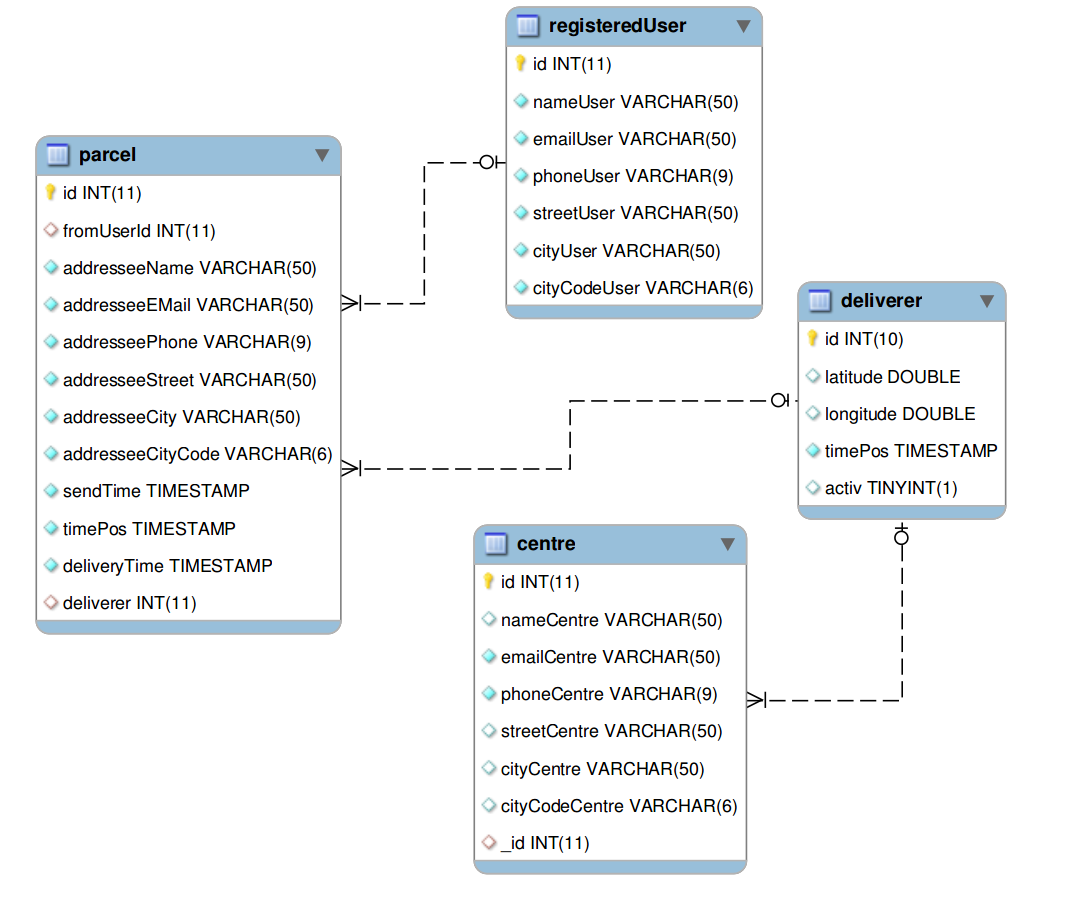
\includegraphics[width=0.9\textwidth]{ERD.png}
\caption{Diagram ERD zaprojektowanej bazy danych}
\label{fig:ERD}
\end{figure}

Na rysunku \ref{fig:ERD} przedstawiono diagram ERD pokazujący tabele oraz
połączenia pomiędzy tabelami. Każda z tabel ma swój klucz główny \texttt{id}. Tabela
\texttt{parcel} (przesyłka) zawiera w sobie dwa obce klucze (\texttt{foreign
key}) odwołują się one do: \texttt{deliverer.id} - klucz główny
tabeli kurier oraz \texttt{registeredUser.id} - klucz główny tabeli użytkownika zarejestrowanego,
czyli tego który złożył zamówienie na przesyłkę. Tabela centre, która ma
zawierać wpisy dotyczące nazwy, ulicy, miasta zawiera w sobie obcy klucz do
tabeli deliverer. Wybrano takie rozwiązanie ponieważ w tabeli \texttt{deliverer}
są podawane długość i szerokość geograficzna, które w łatwy sposób powiązano z
tabelą \texttt{centre}.

\chapter{Przygotowanie i uruchomienie aplikacji}

Do utworzyć opisywany w tej pracy projekt należy zacząć od instalacji IDE
Eclipse,  najprościej jest zacząć od instalacji Eclipse ADT z dodatkiem Android
SDK \cite{eclipse}, po jego instalacji w widoku Eclipse pojawi się ikona
,,Android SDK Manager''. Po załadowaniu się menedżera należy wybrać co najmniej
SDK Tools, SDK Platform-tools, SDK Build-tools (najwyższą dostępną wersję), oraz w
folderze z ostatnią wersją systemu Android X.X zaznaczyć SDK Platform i
emulator do obrazu systemu Android (ARM EABI v7a System Image), ponadto na
potrzeby tego projektu konieczne jest zainstalowanie Google Repository i Google
Play Services z folderu Extras.

Następnym krokiem jest zainstalowanie serwera Apache Tomcat w IDE Eclipse.
Dodanie serwera realizuje się od otworzenia zakładki
Window>Preferences>Server>Runtine Enviroment i tam należy dodać (add) Apache
Tomcat również w najnowszej wersji. Serwer będzie już wtedy zainstalowany. 

Autor korzysta z systemu operacyjnego Linux dystrybucja Ubuntu, więc zostanie
opisana instalacja \emph{\color{komentarz}\ldots Darku opisz, ja nie wiem jak,
bo Ty mi to zrobiłeś :*}

Jeśli w IDE Eclipse nie ma dodanych odpowiednich perspektyw trzeba je dodać
(Open Perspective) będzie potrzebna perspektywa ,,Java'' oraz ,,SQL Explorer''.
Po spełnieniu wszystkich poprzednio wymienionych kroków można eksportować
projekty. Import projektów wybiera się w zakładce File>Import>Editing Project
Into Workspace.

\chapter{Wykorzystane technologie}

Zrealizowany tu projekt bazuje na nowoczesnych technologiach.
Skorzystano z mobilnego urządzenia - telefonu komórkowego z systemem
Android, bazy danych do przechowywania informacji, a także serweru, który to
łączy wszystkie elementy w jedną spójną całość. Głównym językiem
programowania wykorzystanym w projekcie jest język Java, dzięki któremu
zrealizowano aplikację mobilną, obsługę Servletu, bazy danych, odpytywania i
parsowania odpowiedzi serwera Google o widok mapy i odległości pomiędzy dwoma
punktami, a także obsługa witryny http. Całą aplikację stworzono za pomocą IDE
Eclipse z odpowiednimi dodatkami.

\section{Java}

Java jest obiektowym językiem programowania ogólnego przeznaczenia.
Charakteryzuje się silnym ukierunkowaniem na obiektowość oraz niezależnością i
przenoszalnośćią kodu od architekty.Oprócz wyżej wymieniowych założeniami języka
Java jest prostota, sieciowość, niezawodność, bezpieczność, interpretowalność, wysokowydajny,
wielowątkowy, dynamiczny oraz niezależny od architektury. 

\begin{itemize}
  \item  \parbox[t]{\dimexpr\textwidth-\leftmargin}{
      \vspace{-2.5mm}
    \begin{wrapfigure}{R}{0.3\textwidth}
	\centering
	
\includegraphics[width=0.18\textwidth]{javaEE.png}
	\caption{\label{fig:javaEE}Logo Java EE.}
	\end{wrapfigure}
  Prosty - założeniami autorów języka Java było aby programista bez
  specjalnych szkoleń mógł od razu zacząć pisać w języku Java. Składnia została
  oczyszczona (w stosunku do C++) o arytmetykę wskaźnikową, struktury, unie,
  przeciążanie operatorów itd. 
	}
  \item Zorientowany obiektowo;
  \item Sieciowy - Java posiada bibliotekę, która w przystępny sposób umożliwia
  pracę z protokołami http, TCP/IP, FTP;
  \item Niezawodny - szczególnie skupiono się na wykrywaniu ewentualnych
  problemów, zapobieganiu sytuacjom, w których może błąd nastąpić oraz
  sprawdzaniu błędów podczas działania programu;
  \item Bezpieczny - Java może służyć do zastosowań sieciowych, z tego powodu
  zadbano o możliwe najlepsze zabezpieczenie przed wirusami i ingerencja osób
  trzecich;
  \item Niezależny od architektury - Java kompilowana jest do kodu pośredniego
  (bajtowego), który następnie jest interpretowany na maszynie wirtualnej Javy,
  która jest dostosowana do odpowiedniego systemu. Maszyna wirtualna Javy(JVM)
  jest zdolna wykonywać program z kodu pośredniego. Z tego powodu jeżyk Java
  stosowany jest na wielu urządzeniach oraz różnych systemach operacyjnych.
  Niestety konsekwencją przenoszalności kodu jest jego wolniejsze wykonanie;
  \item Przenośny - Java posiada ściśle określone rozmiary typów danych i nie ma
  możliwości zmiany rozmiaru przez programistę przez co nie następuje np. zmiana
  kolejności bajtów;
  \item Interpretowany - program nie jest kompilowany tylko przechowywany w
  postaci kodu źródłowego, podczas uruchomienia zostaje dopiero interpretowany i
  uruchamiany przez interpreter języka;
  \item Wysokowydajny - istnieje możliwość tłumaczenia kodu bajtowego w locie,
  co zwiększa szybkość ładowania się programu;
  \item Wielowątkowy - pozwala na interaktywność między procesami, a także pracę
  w czasie rzeczywistym;
  \item Dynamiczny - obiekty w Javie można zmieniać w zależności od
  zmieniającego się środowiska oraz możliwy jest wgląd we wszystkie obiekty, a
  nawet dodawać nowe metody;
\end{itemize}

Język Java wywodzi się z języków C++ i C, wykorzystuje wiele potrzebnych i
użytecznych funkcjonalności tych języków, z nieużytecznych, trudnych lub
powodujących często błędy zrezygnowano. Język Java umożliwia dziedziczenie, a
ponadto wszystkie obiekty Javy są pochodną obiektu bazowego. Jednakże Java nie
umożliwia dziedziczenia wielobazowego, dlatego do Javy wprowadzono interfejsy -
abstrakcyjny typ, który posiada jedynie operacje, ale nie posiada danych, z tego
powodu można tylko implementować interfejs i nie można utworzyć obiektów tego
typu. Język Java umożliwia pisanie aplikacji stacjonarnych, webowych czy
mobilnych. Język Java ma rozbudowaną obsługę wyjątków. Posiada dobrze
rozbudowanego \texttt{GarbageCollector} (odśmieciacza) \cite{java.doc}.

\section{Wzorzec architektoniczny - MVC}

W projekcie do zorganizowania struktury aplikacji serwerowej został zastosowany
wzorzec architektoniczny MVC (Model-View-Controller). W modelu tym Model jest
odpowiedzialny za przechowywanie logiki, z której korzystają inne składowe
systemu. Kolejną częścią składową tej struktury jest Widok, który to jest
odpowiedzialny za funkcje prezentacji w ramach interfejsu użytkownika, ale
także może posiadać swoją logikę. Ostatnim elementem systemu jest Kontroler,
który spaja dwie wcześniejsze części. Kontroler odpowiada za przepływ danych
od/do użytkownika, reakcję systemu w zależności od zachowania użytkownika,
kontroler także zarządza Modelem i Widokiem. Takiej strukturze jest jasno
zdefiniowane, która część systemu pełni jakie funkcje. Taka struktura
architektoniczna jest najczęściej stosowana w aplikacjach www, gdzie widać
wyraźną granicę pomiędzy widokiem i modelem, a kontrolerem jest serwer, który
obsługuje informacje płynące z widoku (z http), odpowiednio formuje model i
przekazuje go do widoku. \cite{java.mvc}

\begin{figure}[ht!]
\centering
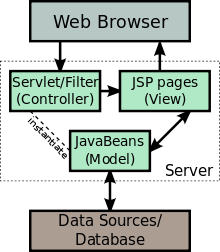
\includegraphics[width=60mm]{jspModel.png}
\caption{Schemat systemu Model-View-Controller model 2\cite{java.mvc.grafika}}
\label{fig:MVC2}
\end{figure}

Autor w swojej pracy użył modelu MVC2 [rys. \ref{fig:MVC2}]
Uzasadnieniem użycia tego wzorca jest ułatwiona organizacja aplikacji, w której
istnieje interfejs graficzny użytkownika. Dzięki niemu w prosty logiczny sposób
można było rozdzielić logikę, kontrolę i widok. Kontrolerem z [rys.
\ref{fig:MVC2}] jest opisany w kolejnym podrozdziale Servlet.

\newpage
\section{Servlet}

Servlet są to aplikacje działające na serwerze WWW korzystające z języka Java.
Serwlety mają zapewniać budowanie aplikacji internetowych niezależnych od
platformy. Servlet umożliwia korzystanie z baz danych i http. Z tego powodu
wykorzystywane są do budowania interaktywnych aplikacji internetowych. 

\begin{wrapfigure}{r}{0.3\textwidth}
\centering
\subfigure {

\includegraphics[width=10ex]{feather.png}

\includegraphics[width=10ex]{tomcat.png}
}
\caption{\label{fig:apache}Logo Apache i Apache Tomcat.}
\vspace{-35pt}
\end{wrapfigure}

Serwer Apache obsługuje www za pomocą protokołu. Wybrana w projekcie dystrybucja
to Servlet Tomcat Apache [rys. \ref{fig:apache}], który jest http, jest otwarty,
zapewnia wielowątkowość, skalowalność, bezpieczeństwo oraz kontrolę dostępu
\cite{apache.wiki}.

Wybór Tomcat Apache na serwer podyktowany był przez wybór jako głównego języka
aplikacji - Javy. Servlet jest dość popularnym narzędziem, co pomogło także w
uruchomieniu i skonfigurowaniu go.

\section{JSP - Java}

JSP (ang. JAvaServer Pages) jest to technologia, dzięki której możliwe jest
dynamiczne tworzenie stron webowych. JSP bazuje na językach znacznikowych, np.
HTML, xml oraz innych. Technologia ta jest kompatybilna z servletami (Apache
Tomcat, i innymi).

To właśnie wprowadzenie plików JSP wymaga korzystanie z wcześniej
opisanego modelu MVC [rys. \ref{fig:MVC2}]. W dodatku JSP oprócz użycia języków
skryptowych umożliwia przeplatanie ich z językiem Java. Wtedy kod, który będzie
napisany w Javie musi być wzięty w znaki <\% \ldots \%>, np. fragment z listingu
\ref{lst:Sprawdz.jsp}:

\texttt{<\% out.print("Nadawca"); \%> \$\{regUserName\}
\$\{regUserAddr\}}

Natomiast frazy ujęte w znaki \$\{\ldots\} służą do dostępu (pobrania
i/lub wysyłania) do danych i funkcji, które powstały w obiektach Javy. Żeby
przekazać taką wartość z klasy Javy, klasa ta musi rozszerzać Servlet
(\texttt{extends HttpServlet}) ustawiać taki parametr jaki jest pomiędzy
nawiasami \{\} korzystając z HttpServletRequest, jako przykład podano fragment z
listingu \ref{lst:Sprawdz.doPost.java}:

\texttt{req.setAttribute("regUserName",
						searchParcel.getRegisteredUserNameUser());}

\section{Technologie internetowe}

W przedstawionym w tej pracy projekcie korzystano z technologi internetowych,
które obsługiwały interakcję z użytkownikiem oraz `strony www`. Skorzystano
z takich technologii jak:
\begin{itemize}
  \item JavaScript - jest to skryptowy język programowania stosowany głównie do
  tworzenia stron internetowych, zapewnia interakcję z
  użytkownikiem\cite{javascript.wiki}, służy do kontroli przeglądarki, zmiany
  treści strony. Składnia języka JavaScript jest zbudowana na podstawie języka
  C. Język umożliwia dynamiczne typowanie oraz jest obiektowy;
  \item HTML - jest to jeżyk znaczników służący do tworzenia stron
  internetowych. Język składa się z tagów umieszczonych w \texttt{<tag>},
  elementy, np. napisy, umieszane są pomiędzy tagami \texttt{<tag> napis
  </tag>}, gdzie pierwszy znacznik jest tagiem oznaczającym początek, a drugi
  zamykającym. HTML jest budulcem strony internetowej, opisuje jej strukturę.
  HTML można osadzać w takich językach jak JavaScript, może odnosić się do
  stylów CSS, który służy do definiowania wyglądu i układu tekstu i innych na
  stronie;
  \item XML - jest to język znaczników przeznaczony do reprezentowania danych w
  strukturyzowany sposób \cite{xml.wiki}. Tak jak HTML składa się ze znaczników
  <\ldots> i </\ldots> i tagów.
  \item Protokół http - jest podstawą do komunikacji danych w WWW, służy do
  wymiany i przesyłania. Funkcjonuje w trybie żądanie-odpowiedź w
  modelu klient-serwer, gdzie przykładowo przeglądarka jest klientem, a
  aplikacja uruchomiona na komputerze serwerem. HTTP jest protokołem warstwy
  aplikacji, która zapewnia komunikację.
  \item \ldots
\end{itemize}

\newpage
\section{db - MySQL}

W projekcie do przechowywania danych skorzystano z baz danych. Baza danych
pozwala w ustrukturyzowany sposób kolekcjonować dane niezbędne do działania
programów. Przechowywane dane mogą być o dowolnym formacie i strukturze.

Systemem, do zarządzania bazą danych w projekcie był MySQL. MySQL jest
rozwijany przez firmę ORacle. Jest opensource'owe rozwiązanie do zarządzania
relacyjnymi bazami danych. Charakteryzuje się takimi cechami jak szybki,
wielowątkowy dostęp z możliwością obsłużenia dużej ilości użytkowników. Serwer
MySQL może być stosowany do systemów, w których znajdują się dane o znaczeniu
krytycznym lub te systemy są mocno obciążane \cite{Mysql.com}. 

Język MySQL posiada takie typy danych jak signed/unsigned int, long, float,
double, char, varchar, date, time, datetime, enum i inne. Język MySQL składa się
z takich typów komend jak: DML (ang.
Data Manipulation Language - dotyczące manipulowania), DLL (ang. Data
Defitnition Language) oraz DCL (ang. Data Control Language).
Komendy DML:
\begin{itemize}
  \item \texttt{select} - służy do otrzymywania wierszy z wybranych tabeli,
  najpopularniejsza forma użycia komendy \texttt{select}:
    
  \texttt{SELECT select\_expr [, select\_expr] [FROM table\_name] [WHERE
  where\_condition];}
  
  \item \texttt{insert} - komenda ta wstawia nowe wiersze do istniejącej tabeli,
  istnieją trzy przypadki użycia tej komendy:
  
  \texttt{INSERT [INTO] table\_name [(col\_name,...)]
    {VALUES | VALUE} ({expr | DEFAULT},...),\newline (...), ...
    [ ON DUPLICATE KEY UPDATE
      col\_name=expr
        [, col\_name=expr] ... ];} 
  
  \texttt{INSERT [INTO] table\_name SET col\_name={expr | DEFAULT}, ... [ ON
  DUPLICATE KEY \newline UPDATE col\_name=expr [, col\_name=expr] ... ];}
      
   \texttt{INSERT [INTO] table\_name [(col\_name,...)]
    SELECT ... \newline[ ON DUPLICATE KEY UPDATE
      col\_name=expr
        [, col\_name=expr] ... ];}
  
  \item \texttt{update} - aktualizuje kolumny istniejących wierszy,
  struktura użycia komendy:
  
  \texttt{UPDATE table\_name
    SET col\_name1={expr1|DEFAULT} [, col\_name2={expr2|DEFAULT}] ...
    \newline[WHERE where\_condition];}
  
  \item \texttt{delete} - usuwa pojedyncze wiersze, użycie komendy:
  
  \texttt{DELETE FROM table\_name [WHERE where\_condition];}
  
  \item i inne
\end{itemize}
Komendy DLL:
\begin{itemize}
  \item \texttt{create} - komenda stosowana w połączeniu z database, function,
  index, procedure, table, trigger, view. Komenda używana jest wtedy gdy chce
  się dodać nową bazę danych czy tabelę. 
  \item \texttt{alter} - komenda używana w połączeniu z database, table,
  function, procedure oraz view. Służy do zmiany struktury bazy danych, tabeli,
  \ldots, np można dodać lub usunąć kolumnę istniejącej tabeli.
  \item \texttt{drop} - umożliwia usunięcie bazy danych i tabeli
\end{itemize}
Komendy DML:
\begin{itemize}
  \item \texttt{commit} - komituje wpisaną transakcję, wprowadzona zmiana jest
  pernamenta,
  \item \texttt{rollback} - wycofuje ostatnią wpisaną transakcję.
\end{itemize}

Oprócz wyżej wymienionych MySQL posiada również inne komendy, jednak są one
znacznie rzadziej wykorzystywane, dlatego nie zostały tutaj przytoczone.

\newpage
\section{Android}

Android jest systemem wykorzystywanym na platformach mobilnych. Android
jest systemem operacyjnym z rodziny Linux, oparty na jądrze Linux. Android
umożliwia tworzenie aplikacji na wiele urządzeń, optymalizacji podlega plik xml,
gdzie można dostosować aplikację do konkretnych urządzeń. Każdy proces
uruchomiony na Androidzie jest uruchamiany na maszynie wirtualnej i jest
niezależny od pozostałych aplikacji. Najnowszą wersją systemu jest Android
Lollipop 5.0.

Rozpoczęcie pracy z Androidem zaczyna się od instalacji środowiska, może to być
Eclipse z dodatkiem SDK Android lub Android Studio. A samo tworzenie aplikacji
od projektu interfejsu użytkownika, następnie dopiero oprogramowuje się
obsługę oraz logikę aplikacji, ostatnim etapem jest testowanie aplikacji
\cite{developer.android}.

System Android składa się z czterech podstawowych elementów. 

\begin{itemize}
  \item Activites - reprezentuje ekran użytkownika, np. aplikacja do obsługi
  emaila posiada jedną aktywność do listowania nowych emiali, a inną
  do pisania email. Aktywności implementuje się używając
  podklasę \texttt{Activity};
  \item Services - jest to składnik aplikacji, który działa w tle, np. w
  urządzeniu odtwarzana jest muzyka w tle, a użytkownik korzysta z innej
  aplikacji w tym czasie. Takie zachowanie aplikacji implementuje się za pomocą
  podklasy \texttt{Service};
  \item Content providers - służy do zarządzania wspólnymi danymi, a także
  danymi, które są prywatne dla danej aplikacji. Zarządzanie danymi
  implementuje się używając podklasy \texttt{ContentProvider};
  \item Broadcast receivers - jest komponentem systemu, który jest
  odpowiedzialny za rozgłaszanie informacji po systemie, np. informacja o
  niskim stanie baterii. Taką właściwość implementuje się korzystając z podklasy
  \texttt{BroadcastReceiver}.
\end{itemize}

Wartą częścią do roziwnięcia jest element \texttt{Activity}. \texttt{Activity}
jak już wcześniej wspomniano jest reprezentuje ekran użytkownika. Ekran oferuje
współdziałanie z użytkownikiem, zazwyczaj okno aplikacji wypełnia cały ekran,
ale może być tak naprawdę każdego rozmiaru, także może być pływające na wierzchu
inncyh okien. 

Taka aplikacja składa się z wielu cześci, które są ze sobą
powiązane w luźny sposób. Zazwyczaj jedna część aplikacji jest ,,główna'',
najczęściej ta, która jest pokazywana użytkownikowi przy uruchomieniu aplikacji.
Następnie każde działanie wykonane na tym ekranie może uruchamiać inny ekran,
proces czy działanie. Wtedy przy każdym uruchomieniu nowej działaności ,,stara''
jest zatrzymywana i przechowywana na stosie - LIFO (ang. last in first out).
Dzięki temu gdy użytkownik zapragnie wrócić do poprzedniej działaności (ekranu)
przyciska przycisk wstecz i poprzednia działaność jest zdejmowana ze stosu.

Utworzenie aplikacji typu \texttt{Activity} wymaga utworzenie podklasy
\texttt{Activity}, w tej podklasie należy zaimplementować metody, które będą
określały aplikację pomiędzy różnymi stanami cyklu jej życia. Mówiąc cykl życia
aplikacji ma się na myśli tworzenie, zatrzymywanie, wznawianie, niszczenie.
Najważniejszymi metodami do zaimplementowania są zatem metody
\texttt{onCreate()} oraz \texttt{onPause()}. Metoda \texttt{onCreate()} jak sama
nazwa wskazuje, określa stan aplikacji podczas jej tworzenia, natomiast metoda
\texttt{onPause()} określa co się stanie z aplikacjią jeśli opuści ją użytkownk,
co nie musi oznaczać, że aplikacja zostanie zakończona, zazwyczaj zachowywany
jest wtedy aktualny stan.

Oczywiście istotną kwestią jest zarządzanie życiem aplikacji. Aktywność może być
zatem w jednym z trzech stanów: stan wznawiania, wstrzymanie oraz
zatrzymania. Stan wznawiania określa stan aplikacji kiedy jest ona włączona i
jest na głownym planie ekranu użytownika - ,,działa''. Stan wstrzymania dotyczny
stanu, w którym aplikacja jest widoczna, ale nie jest na górze, może być
częściowo widoczna na ekranie. Stan zatrzymania oznacza, że aplikacja jest
całkowicie przysłonięta przez inne i działa w tle. W stanie wstrzymania i
zatrzymania system w przypadku braku pamięci może zatrzymać aplikację.

Na rysunku \ref{fig:andActivityLifecycle} przedstawiony został cykl życia
aplikacji. Wspomniana metoda \texttt{onCreate()} tworzona jest zawsze wtedy, gdy
aplikacja jest tworzona, w tym miejscu tworzy się widoki. Następną
wywoływaną metodą jest \texttt{onStart()} powoduje pokazanie się aplikacji pod
restarcie lub zatrzymaniu aplikacji. Metoda \texttt{onResume()} wywoływana jest
zawsze po pauzie aplikacji i rozpoczyna interakcję z użytkownikiem, przywołuje
aplikację na szczyt stosu. \texttt{onPause()} wywołwana w momencie, gdy
aplikacja ma rozczpocząć inną czynność. Metoda \texttt{onStop()} zostaje użyta,
gdy aplikacja ma się stać niewidoczna dla użytkonika, aplikacja po tym może być
zniszczona, może zostać zamknięta jej aktywność lub może być zrestartowana.
Ostatnią metodą przez zniszczeniem aplikacji jest \texttt{onDestroy()}, która
jest metodą ostatnią jaka może zostać wykonana, wszystkie procesy są zamykane.

\begin{figure}
\centering
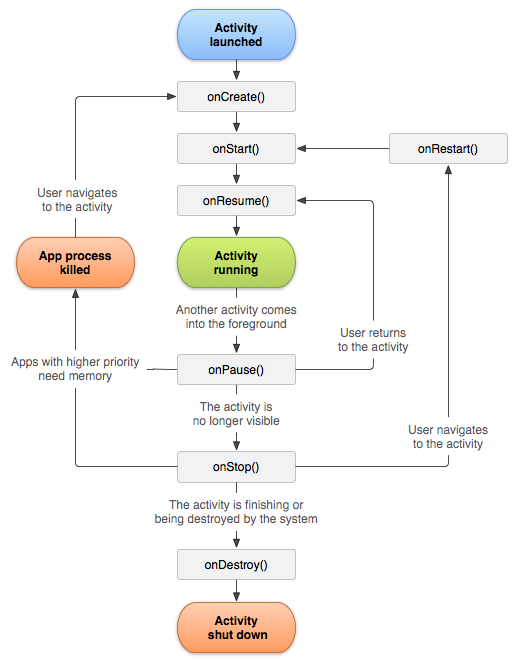
\includegraphics[width=0.55\textwidth]{andActivityLifecycle.png}
\caption{Schemat cyklu życia aplikacji\cite{developer.android}}
\label{fig:andActivityLifecycle}
\end{figure}

Przedstawiony na rysunku \ref{fig:andActivityLifecycle} schemat cyklu życia aplikacji w systemie
Android jest oczwywiśćie podstawowy i może posiadać więcej funkcji, jednakże jest to ogólny
schemat budowania aplikacji typu \texttt{Activity}.

\section{Google apps - mapy}

Firma Google udostępnia korzystanie deweloperom ze swoich produktów
\cite{developer.google}. W swoim projekcie korzystałam z Google Maps API. 

\chapter{Możliwość rozwinięcia w przyszłości}
Aplikację można „podpiąć” pod prawdziwe urządzenia jakie posiadają kurierzy – te na których się człowiek podpisuje – ale konieczne będzie 
zrefakturyzowanie(?)/zmianie kodu pod system, który mają tam zainstalowany.
	Fajnie by było to wrzucić na prawdziwe tablety, można by sprzedawać/zarobić. Ogólnie koszt takiego urządzenia to byłoby tablet/telefon 
	+ wycena za program.
	Normalnie kurierzy używają kolektorów danych.
	
	
 Nie tylko GPS do lokalizacji, bo także odbicia
na czytnikach u kurierów Projekt opiera się 

\chapter{Wnioski i podsumowanie}
\addcontentsline{toc}{chapter}{Bibliografia} %utworzenie w spisie tresci pozycji Bibliografia
\bibliography{bibliografia} % wstawia bibliografie korzystajac z
% pliku bibliografia.bib - dotyczy BibTeXa, jezeli nie korzystamy z BibTeXa nalezy uzyc otoczenia thebibliography

%opcjonalnie moze sie tu pojawic spis rysunkow i tabel
\listoffigures
\lstlistoflistings
\end{document}
